% !TEX program = lualatex
% !TEX encoding = UTF-8 Unicode
% 
\newcommand{\titol}{Estimación de la cardinalidad}
\newcommand{\materia}{Algorítmica}
\newcommand{\idioma}{english,spanish}
\newcommand{\pdfauthors}{Héctor Ramón Jiménez, Xavier Serra Alza}
\newcommand{\autors}[1]{\begin{tabular}{#1} Ramón -- Serra\end{tabular}}
\newcommand{\data}{\today}
% !TEX encoding = UTF-8 Unicode
% !TEX root = report.tex
% 
\documentclass[a4paper,11pt,twoside,titlepage,abstract,numbers=noenddot,automark,mnsy,intlimits,rgb,dvipsnames]{scrartcl}
%\usepackage[utf8]{inputenc}
\usepackage{csquotes}
\usepackage[\idioma, es-tabla]{babel}
\spanishdecimal{.}
\usepackage{fontspec}
\defaultfontfeatures{Scale=MatchLowercase, Ligatures=TeX}
\usepackage{pdfpages}
\usepackage{fancyvrb}
\usepackage{amssymb}
\usepackage{amsmath}
\usepackage{mathtools}
\usepackage{unicode-math}
\unimathsetup{math-style=ISO,vargreek-shape=unicode}
\usepackage{xunicode}
\usepackage{ifxetex}
\usepackage{algorithm}
\usepackage{algpseudocode}

\ifxetex
  \usepackage{xltxtra}
\fi
\usepackage{verbatim}

\usepackage[binary-units]{siunitx}
\sisetup{
  product-units=single,
  list-units=single,
  per-mode=symbol,
  list-final-separator = { y },
  list-pair-separator = { y },
  range-phrase = { a },
}

\usepackage{fullpage}
\usepackage{framed}
\usepackage{xfrac}

\defaultfontfeatures{Scale=MatchLowercase}
\setmainfont[Ligatures=TeX,
BoldFont=texgyrepagella-bold.otf,
BoldItalicFont=texgyrepagella-bolditalic.otf,
ItalicFont=texgyrepagella-italic.otf]{texgyrepagella-regular.otf}
\setsansfont[Ligatures=TeX,
BoldFont=lmsans10-bold.otf,
BoldItalicFont=lmsans10-boldoblique.otf,
ItalicFont=lmsans10-oblique.otf]{lmsans10-regular.otf}
\setmonofont[BoldFont=lmmonolt10-bold.otf,
BoldItalicFont=lmmonolt10-boldoblique.otf,
ItalicFont=lmmono10-italic.otf,
SlantedFont=lmmonoslant10-regular.otf]{lmmono10-regular.otf}
\setmathfont{texgyrepagella-math.otf}
\setmathfont[range={\mathcal,\mathbfcal},StylisticSet=1]{xits-math.otf}

\usepackage[super]{nth}
%\setmathfont[ Path=fonts/, ]{LM Math}
%\usepackage{natbib}
\usepackage[natbib=true,language=english,style=numeric,citestyle=numeric,bibstyle=numeric,hyperref=true]{biblatex}

\usepackage{url}
\usepackage{pdflscape}
\usepackage{enumitem}

\usepackage{graphicx}
\usepackage{float}
\usepackage{caption}
\usepackage{subcaption}
\usepackage{multicol}
\usepackage{booktabs}

\usepackage[hidelinks]{hyperref}
\hypersetup{
    pdfencoding=auto,
    pdffitwindow=false,      % page fit to window when opened
    pdftitle={\materia\ :: \titol},    % title
    pdfauthor={\pdfauthors},     % author
    pdfsubject={},   % subject of the document
    pdfcreator={XeLaTeX + Hyperref package},
    colorlinks=false
}

\usepackage{setspace}

\usepackage[nouppercase]{scrpage2}

\setlength{\headheight}{15pt}
\renewcommand{\headfont}{\upshape}
\defpagestyle{curr}
  {    %% superior
    (\textwidth,0pt) %líneas
    {    %%par
      {\autors{l}}
      {\hfill}
      {\leftmark}
    }
    {	%%impar
      {\rightmark}
      {\hfill}
      {\autors{r}}
    }
    {	%% una sola cara
      {\thepart}
      {\hfill}
      {\autors{r}}
    }
    (\textwidth,0.5pt) %líneas
  }
  {		%% inferior
    (\textwidth,0.5pt) %líneas
    {	%%par
      {\thepage}
      {\hfill}
      {\materia}
    }
    {	%%impar
      {\titol}
      {\hfill}
      {\thepage}
    }
    {	%% una sola cara
      {\materia: \titol}
      {\hfill}
      {\thepage}
    }
    (\textwidth,0pt) %líneas
  }

\pagestyle{curr}

\headsep = 15pt
%\addtolength{\footskip}{-16pt}
%\addtolength{\textheight}{+16pt}
\addtolength{\topmargin}{-15pt}
\addtolength{\hoffset}{12mm}
\addtolength{\textwidth}{-11mm}
\usepackage{wrapfig}

\usepackage{amsthm}
%~ \theoremprework {\textcolor{white} {\rule{0.2in}{0.11in}} \hrule\rule{0.2in}{0.11in}}
%~ \theorempostwork {\hrule %\textcolor{white} {\rule{0.2in}{0.11in}}
%~ }

\makeatletter
\newcommand{\strong}[1]{\@strong{#1}}
\newcommand{\@@strong}[1]{\textbf{\let\@strong\@@@strong#1}}
\newcommand{\@@@strong}[1]{\textnormal{\let\@strong\@@strong#1}}
\let\@strong\@@strong
\makeatother

%~ \theoremindent0.5cm
%~ \theoremstyle{break}
%~ \theorembodyfont{}
%~ \newtheorem*{defi}{}

\theoremstyle{plain}% default
\newtheorem{thm}{Teorema}[section]
\newtheorem{lem}[thm]{Lemma}
\newtheorem{prop}{Proposition}
\newtheorem{cor}{Corollary}

\theoremstyle{definition}
\newtheorem{defn}{Definition}[section]
\newtheorem{conj}{Conjecture}[section]
\newtheorem{exmp}{Example}[section]

\theoremstyle{remark}
\newtheorem*{obs}{Observation}
\newtheorem*{note}{Remark}
\newtheorem{case}{Case}
\newtheorem*{notation}{Notation}

\addtolength{\voffset}{-15pt}
\addtolength{\headsep}{10pt}
\addtolength{\textheight}{35pt}
\addtolength{\footskip}{-20pt}
\addtolength{\textwidth}{15pt}
\addtolength{\marginparwidth}{-20pt}
\addtolength{\oddsidemargin}{-20pt}
\addtolength{\evensidemargin}{-20pt}

\usepackage{listings}

\definecolor{FonsCodi}{cmyk}{0,0,0,0.04}
\definecolor{Comentaris}{cmyk}{0,0,0,0.6}
\definecolor{mygreen}{rgb}{0,0.6,0}
\definecolor{mygray}{rgb}{0.6,0.6,0.6}
\definecolor{mymauve}{rgb}{0.58,0,0.82}
\definecolor{darkgreen}{rgb}{0.2,0.5,0.2}
\definecolor{orange}{rgb}{1,0.5,0}

\lstset{ %
basicstyle=\ttfamily\small,
numbers=none,                   % where to put the line-numbers
backgroundcolor=\color{FonsCodi},  % choose the background color. You must add \usepackage{color}
rulesepcolor=\color{FonsCodi},
lineskip=-2.5pt,
showspaces=false,               % show spaces adding particular underscores
showstringspaces=false,         % underline spaces within strings
showtabs=false,                 % show tabs within strings adding particular underscores
frame=single,                    % adds a frame around the code
tabsize=8,	                % sets default tabsize to 2 spaces
captionpos=t,                   % sets the caption-position to top
breaklines=true,                % sets automatic line breaking
breakatwhitespace=true,        % sets if automatic breaks should only happen at whitespace
escapeinside={\%*}{*)},          % if you want to add a comment within your code
columns=flexible
}

\renewcommand{\lstlistlistingname}{Lista de ejecuciones}
\renewcommand{\lstlistingname}{Ejecución}

\setstretch{1.0}
\DefineBibliographyStrings{spanish}{%
  references = {Referencias},
}

\title{\materia\\
\Large{\titol}}
\subtitle{Facultat d'Informàtica de Barcelona\\ % Pongo la I mayúscula porque la FIB lo hace
Universitat Politècnica de Catalunya}
\author{
  Héctor Ramón Jiménez \\
  Xavier Serra Alza}
\date{
  \today \\
  cuatrimestre de otoño \\
  curso 2013--2014}

\everymath{\displaystyle}

\newcommand{\CC}{\mathbb{C}}
\newcommand{\RR}{\mathbb{R}}
\newcommand{\NN}{\mathbb{N}}
\newcommand{\bigO}[1]{\ensuremath{\operatorname{O}\left(#1\right)}}% big-O notation/symbol
\newcommand{\bigOmega}[1]{\ensuremath{\operatorname{\Omega}\left(#1\right)}}% big-O notation/symbol
\newcommand{\bigTheta}[1]{\ensuremath{\operatorname{\Theta}\left(#1\right)}}% big-O notation/symbol
\newcommand{\slot}[1]{\textsl{\texttt{#1}}}
\newcommand{\clase}[1]{\texttt{#1}}
\newcommand{\regla}[1]{\textsl{\textsf{#1}}}

\newenvironment{slotlist}{%
   \renewcommand\descriptionlabel[1]{\hspace{\labelsep}\slot{##1}}
   \begin{description}%
}{%
   \end{description}%
}

\bibliography{references}
\begin{document}

\renewcommand{\listalgorithmname}{Índice de algoritmos}

\maketitle
\tableofcontents
\listofalgorithms
\listoftables
\listoffigures
\vfill
\cleardoublepage

% !TEX encoding = UTF-8 Unicode
% !TEX root = ../report.tex
% 
\section{Introduccion}
[...]

% !TEX encoding = UTF-8 Unicode
% !TEX root = ../report.tex
% 
\section{Investigación}

La información referente al algoritmo \texttt{HyperLogLog} se ha obtenido principalmente
del artículo \citetitle{hll:HyperLogLog} ~\cite{hll:HyperLogLog}.
El artículo presenta una descripción detallada del algoritmo y sus ventajas en relación a otros
algoritmos de estimación de cardinalidad.

En esta sección se introducen y se explican, de manera general, las bases del algoritmo \texttt{HyperLogLog}.

\subsection{Funciones de hash}
\label{hash}

Una \textbf{función de hash} se define como una función que mapea todo elemento de un
conjunto de tamaño arbitrario $A$ con otro elemento de un conjunto de tamaño finito $B$.
$$f: A \rightarrow B$$

Una \textbf{buena} función de hash debe ser lo más \textbf{uniforme} posible, es decir, debe mapear los elementos de
$A$ tan \textbf{equitativamente} como sea posible sobre $B$. En otras palabras, todo elemento en $B$ debe ser generado
por la función de hash con \textbf{aproximadamente la misma probabilidad}.

Por lo tanto, si $h$ es una buena función de hash:
$$h: \Sigma^* \rightarrow \{0,1\}^r$$

Donde $\Sigma^*$ representa el conjunto de todas las palabras y $\{0, 1\}^r$ es el conjunto de cadenas binarias de $r$ bits.
Entonces, dada una palabra cualquiera $w \in \Sigma^*$, se puede esperar que:

\begin{align*}
  \left.\begin{array}{r@{\mskip\thickmuskip}l}
    p, a \in \{0, 1\} \\
    p \neq a \\
    1 \leq k \leq r
  \end{array} \right\}
  \quad \implies \quad
  \left.
    P\left( h(w) = p^{k-1} \: a \: b_{k+1} \: b_{k+2} \; ... \; b_r \right) = 2^{-k}
  \right.
\end{align*}

Esto significa que la probabilidad de que la \textbf{primera ocurrencia} de $1$ o $0$ en $h(w)$ sea en el bit $k$ es $2^{-k}$.
Es decir, hay un 50\% de probabilidades de que $h(w)$ empiece por 1, un 25\% de que empiece por $01$, un 12.5\% de que
empiece por $001$, y así sucesivamente.

\subsection{Descripción general del algoritmo}
\label{investigacion:descripcion}

La idea principal de \texttt{HyperLogLog} gira en torno a la propiedad de \textbf{uniformidad} que presentan las buenas
funciones de hash.

Dada una buena función de hash $h$ (igual que en la sección \ref{hash}):
$$h: \Sigma^* \rightarrow \{0,1\}^r$$

Y si el multiconjunto de entrada $M$ tiene $N$ elementos y $n$ elementos únicos, entonces puede esperarse que:

\begin{align*}
  \left.\begin{array}{r@{\mskip\thickmuskip}l}
    p, a \in \{0, 1\} \\
    p \neq a \\
    N \geq 2 \\
    k = \floor{log_2(N)}
  \end{array} \right\}
  \quad \implies \quad
  \left.
    \exists{w \in M}\!: h(w) = p^{k-1} \: a \: b_{k+1} \: b_{k+2} \: ... \: b_r
  \right.
\end{align*}

Por ejemplo, si $M$ tiene \textbf{4 elementos} ($N = 4$) entonces se puede esperar que \textbf{exista uno tal que su hash
empiece por 01}. Si $N = 8$ entonces un elemento debería empezar con la secuencia 001, y así sucesivamente.

Lo interesante, sin embargo, es \textbf{hacerlo a la inversa}.
Sea $a \in \{0, 1\}$ y $k_{max}$ la posición \textbf{más tardía} en la que se ha observado
una ocurrencia de $a$ para todo hash de todo elemento de $M$ entonces se puede estimar que la cardinalidad $n$ de $M$ sea $E = 2^{k_{max}}$.
Por ejemplo, si tras aplicar $h$ a todo elemento de $M$ se observa que la posición más tardía en la que se ha observado un
$1$ es 3 (el elemento empieza con la secuencia $\textbf{001}$), entonces se puede estimar que $n$ es $E = 2^3 = \textbf{8}$ \textbf{elementos}.

Sin embargo, esta estimación es realmente \textbf{imprecisa}. No es difícil ver que con este estimador
\textbf{la cardinalidad se reduce a simples potencias de 2}. Para eliminar esta imprecisión se usa una tabla $T$ de $m$ entradas
para guardar diferentes $k_{max}$, obteniendo el índice $i$ a partir de los primeros $\floor{log_2(m)}$ bits del hash devuelto
y $k_{candidato}$ con los restantes. A partir de $T$ es posible mejorar el estimador anterior:

$$ E = 2 ^ { \frac{1}{m} \sum\limits_{i=0}^{m}\! T[i] } \cdot m $$

Sin embargo, un análisis estadístico realizado por \emph{Flajolet} ~\cite{hll:HyperLogLog} muestra que este estimador
tiene cierta \textbf{tendencia a hacer estimaciones grandes}. Para corregirlo, la estimación se suele multiplicar por la
\textbf{constante 0.79402}, encontrada de manera \textbf{experimental} por el mismo \emph{Flajolet}.
Este estimador es el que utiliza el algoritmo \texttt{LogLog}, una versión anterior a \texttt{HyperLogLog}, el cual tiene
\textbf{un error estándar} de  $\frac{1.30}{\sqrt{m}}$.

\texttt{HyperLogLog} se diferencia del algoritmo \texttt{LogLog} en que aplica la \textbf{media armónica} en vez de la
media aritmética, obteniendo la misma precisión usando solo el $64\%$ de \textbf{memoria que LogLog}, y \textbf{reduciendo así el error estándar} hasta $\frac{1.04}{\sqrt{m}}$.

Por último, si la estimación resultante es muy alta o muy baja entonces se lleva a cabo una corrección:

\begin{description}
\item[Estimación baja] Si $E < \frac{5m}{2}$, se pueden haber dado casos en que haya \textbf{posiciones vacías en la tabla} que
influyan en el valor de la estimación. En éste caso, se cuentan cuantas de estas posiciones vacías
hay, y en caso de que haya por lo menos una, se usa un nuevo valor $E*$ para la estimación: 
$$E* = m \cdot log\left(\frac{m}{V}\right)$$

Siendo $V$ el número de posiciones vacías. Esta fórmula viene dada por las propiedades de las
\textbf{asignaciones aleatorias}. Éstas indican que si $n$ pelotas son lanzadas aleatoriamente a $m$ canastas entonces
se puede esperar que el número de canastas vacías sea $m \cdot e^{-\mu}$, donde $\mu = n / m$. Por tanto, si se observan
$V$ posiciones vacías sobre un total de $m$ es de esperar que $\mu$ sea cercano a $\log(m/V)$, por lo que $n$ estará
cerca de $m \cdot log(m/v)$.

\item[Estimación alta] Asumiendo una función de hash de 32 bits. Si $E > \frac{2^{32}}{30}$, es de esperar que se hayan
producido \textbf{muchas colisiones} que hayan afectado a la estimación final. La corrección consiste en usar la siguiente $E*$
como sustituto de $E$:
$$E* = -2^{32} \cdot log\left(1 - \frac{E}{2^{32}}\right)$$

Para esta fórmula, se usa el mismo modelo de las canastas del punto anterior, pero se sustituye $m$
por $2^r$, siendo $r$ el número de bits usados en la función de hash. Es decir, $E$ \textbf{estima el número de valores diferentes
a los que se les ha aplicado la función de hash}, que será, con una alta probabilidad, próximo a $2^r \cdot (1 - e^{\frac{-n}{2^r}})$.
Y aislando: $n=-2^r \cdot log\left(1 - \frac{E}{2^r}\right)$.
\end{description}

El algoritmo \ref{algoritmo:hyper1} muestra la versión de \texttt{HyperLogLog} descrita en esta sección.

\begin{algorithm}[h!]
\caption{\texttt{HyperLogLog} para funciones de hash de 32 bits}
\label{algoritmo:hyper1}
\textit{Let $h: D\rightarrow \{0,1\}^{32}$ hash data from D to binary 32-bit word.}

\textit{Let $\rho(s)$ be the position of the leftmost 1-bit of s: e.g.,
$\rho(1...) = 1, \rho(0001...) = 4, \rho(0^K) = K + 1$.}

\textbf{define} $\alpha_{16}=0.673;\alpha_{32}=0.697;\alpha_{64}=0.709;\alpha_m=0.7213/(1+1.079/m)$
for $m \geq 128;$

\textbf{Program \texttt{HYPERLOGLOG}} (\textbf{input} $M$: multiset of items from domain $D$).

\textbf{assume} $m=2^b$ with $ b\in[4..16]$.

\textbf{initialize} a collection of $m$ registers, $M[1],...,M[m]$, to 0;

\begin{algorithmic}
    \FOR{$v\in M$}
            \STATE $x  := h(v)$
            \STATE $j   := 1 + (x_1 x_2 ... x_b)_2$ \COMMENT{binary address determined by the first b bits of x}
            \STATE $w := x_{b+1} x_{b+2} ... $
            \STATE $M[j] := max(M[j],\rho(w))$
    \ENDFOR

    \STATE $E:=\alpha _m m^2·\left(\sum\limits_{j=1}^m 2^{-M[j]}\right)^{-1}$ \COMMENT{the raw HyperLogLog estimate}
    \IF{$E \leq \frac{5}{2}m$}
        \STATE $V :=$ the number of registers equal to $0$
        \STATE \algorithmicif\ $V \neq 0$ \algorithmicthen\ $E* := m \cdot log(m / V)$ \algorithmicelse\ $E* := E$
        \COMMENT{small range correction}
    \ENDIF
    \IF{$E\leq \frac{1}{30}2^{32}$}
        \STATE $E*:=E$ \COMMENT{intermediate range -- no correction}
    \ELSE
        \STATE $E* := -2^{32}log(1-E/2^{32})$ \COMMENT{large range correction}
    \ENDIF
    \RETURN{cardinality estimate E* with typical relative error $\pm$ 1.04/$\sqrt{m}$}
\end{algorithmic}
\end{algorithm}

% !TEX encoding = UTF-8 Unicode
% !TEX root = ../report.tex
% 
\section{Implementación}

\subsection{Función de hash}
\label{implementacion:hash}

Para implementar el algoritmo se ha usado una función de hash llamada \texttt{djb2} ~\cite{hash:djb2}.
Se sabe que esta función de hash
es \textbf{muy buena} cuando el \textbf{dominio} es el conjunto de todas las \textbf{cadenas de carácteres ASCII},
hecho que ocurre precisamente en los \textbf{juegos de pruebas disponibles}.

\begin{algorithm}[h]
\caption{Función de hash djb2}
\textbf{let} $a \in \{0, 1\}^{64}$ chosen randomly

\textbf{input} $str \in \Sigma^*$

\textbf{output} $hash \in \{0, 1\}^{64}$
\begin{algorithmic}
    \STATE $hash = 5381$
    \STATE $i := 0$
    \WHILE{$i < length(str)$}
        \STATE $hash := hash * 33 + str[i]$
        \STATE $i := i + 1$
    \ENDWHILE
    \RETURN $a \cdot hash$
\end{algorithmic}
\end{algorithm}

El \textbf{coste temporal} de aplicar esta función de hash a una cadena de cáracteres $str$ es $\bigO{length(str)}$.

La constante $a$ es un número de 64 bits \textbf{escogido aleatoriamente para cada ejecución del programa}.
Esto es necesario para poder realizar un \textbf{estudio estadístico del estimador de cardinalidad} y, además, se evita la posibilidad
de tener juegos de pruebas generados intencionadamente para hacer fallar la estimación, es decir, \textbf{no hay casos peores}.

La función \texttt{djb2} sigue unos principios parecidos a los de un \texttt{Linear Congruental Generator}  (\emph{LCG} para abreviar),
que tiene la forma:
$$X_{n+1} \equiv \left( h \cdot X_n + c \right)~~\pmod{m}$$

Usando $h=33$ y $m=2^{64}$. El valor elegido para $h$ es relativamente arbitrario, pero debe cumplir:

\begin{itemize}
	\item $\textbf{h-1}$ \textbf{es divisible por todos los factores primos de} $\textbf{m}$.
En el caso de $h=33$, $h-1$ es $32$, divisible por el único factor primo de $2^{64}$, el $2$.

	\item $\textbf{h-1}$ \textbf{es múltiplo de 4 si} $\textbf{m}$ \textbf{también lo es}.
En el caso de $a=33$, como $m$ es múltiplo de 4, $h-1$ también lo debe ser, y efectivamente: $32 \! \mod 4 = 0$.
\end{itemize}

Un \emph{LCG} es un algoritmo que produce una secuencia de números \emph{pseudo-aleatorios} calculados mediante una
\textbf{ecuación lineal}. Una de sus principales ventajas es que necesita un \textbf{número muy reducido de bits para mantener el
estado}, por lo que es una buena elección en el entorno en el que se utiliza, donde se dispone de \textbf{poca memoria}.

\subsection{Algoritmo \texttt{HyperLogLog}}
\label{implementacion:algoritmo}

Dado que se ha decidido utilizar una función de hash de 64 bits para minimizar el número de colisiones, resulta innecesario aplicar la
corrección para estimaciones altas vista en la sección: \nameref{investigacion:descripcion} (\ref{investigacion:descripcion}). Esto es así
porque, en la práctica, observar estimaciones cercanas a $2^{64}$ es poco común y, en esos casos, quizás sería mejor utilizar más bits
en la función de hash antes que aplicar la corrección.

El algoritmo \ref{algoritmo:hyper2} muestra en pseudocódigo la versión final que se ha implementado en \texttt{C++} y sobre la que
se ha realizado el análisis estadístico de la sección \ref{analisis}.

\begin{algorithm}[h!]
\caption{\texttt{HyperLogLog} para funciones de hash de 64 bits}
\label{algoritmo:hyper2}
\textit{Let $h: D\rightarrow \{0,1\}^{64}$ hash data from D to binary 32-bit word.}

\textit{Let $\rho(s)$ be the position of the leftmost 1-bit of s: e.g.,
$\rho(1...) = 1, \rho(0001...) = 4, \rho(0^K) = K + 1$.}

\textbf{define} $\alpha_{16}=0.673;\alpha_{32}=0.697;\alpha_{64}=0.709;\alpha_m=0.7213/(1+1.079/m)$
for $m \geq 128;$

\textbf{Program \texttt{HYPERLOGLOG}} (\textbf{input} $M$: multiset of items from domain $D$).

\textbf{assume} $m=2^b$ with $ b\in[4..16]$.

\textbf{initialize} a collection of $m$ registers, $M[1],...,M[m]$, to 0;

\begin{algorithmic}
    \FOR{$v\in M$}
            \STATE $x  := h(v)$
            \STATE $j   := 1 + (x_1 x_2 ... x_b)_2$ \COMMENT{binary address determined by the first b bits of x}
            \STATE $w := x_{b+1} x_{b+2} ... $
            \STATE $M[j] := max(M[j],\rho(w))$
    \ENDFOR

    \STATE $E:=\alpha _m m^2·\left(\sum\limits_{j=1}^m 2^{-M[j]}\right)^{-1}$ \COMMENT{the raw HyperLogLog estimate}
    \IF{$E \leq \frac{5}{2}m$}
        \STATE $V :=$ the number of registers equal to $0$
        \STATE \algorithmicif\ $V \neq 0$ \algorithmicthen\ $E* := m \cdot log(m / V)$ \algorithmicelse\ $E* := E$
        \COMMENT{small range correction}
    \ELSE
        \STATE $E*:=E$
    \ENDIF
    \RETURN{cardinality estimate E* with typical relative error $\pm$ 1.04/$\sqrt{m}$}
\end{algorithmic}
\end{algorithm}

\newpage
% !TEX encoding = UTF-8 Unicode
% !TEX root = ../report.tex
% 
\section{Análisis estadístico del algoritmo}
\label{analisis}

\subsection{Memoria fijada a 1024 bytes}

En esta sección se estudia el comportamiento del algoritmo \texttt{HyperLogLog} en \textbf{9 \emph{datasets}} distintos limitando
la cantidad de memoria utilizada a \textbf{1024 bytes}. En el apéndice \ref{graficas} se incluyen gráficas que muestran los resultados
obtenidos para cada \emph{dataset} de forma detallada. Lo importante, sin embargo, es
\textbf{observar los resultados obtenidos de manera general para cada muestra}.

Se presentan las tablas \ref{tabla:resumen_1024} y \ref{tabla:count_1024} a modo de resumen para cada \emph{dataset}.
\clearpage

\begin{table}[h!]
    \centering
    \begin{tabular}{l r r r S S S}
    \strong{Dataset} & \strong{n} & \strong{N} & \strong{Est. media} &
    \strong{SE} & \textbf{T. medio ($ms$)} & \textbf{T. elem. ($\mu s$)}\\ \hline
    \newcounter{dataset}
\forloop{dataset}{1}{\value{dataset} < 10}{
\textbf{D\arabic{dataset}} &
\input{../data/D\arabic{dataset}/summary_1024.tex}
}
\end{tabular}
    \caption{Memoria fijada a 1024 bytes. Resumen de los resultados.}
    \label{tabla:resumen_1024}
\end{table}

\begin{table}[h!]
    \centering
    \begin{tabular}{l r r r r r r}
    \strong{Dataset} & \strong{[0, 1)} & \strong{[1, 5)} & \strong{[5, 10)} &
    \strong{[10, 15)} & \textbf{[15, 20)} & \textbf{[20, 100]} \\ \hline
\forloop{dataset}{1}{\value{dataset} < 10}{
\textbf{D\arabic{dataset}} &
\input{../data/D\arabic{dataset}/count_1024.tex}
}
\end{tabular}
    \caption{Memoria fijada a 1024 bytes. Clasificación de las ejecuciones según el error relativo (\%).}
    \label{tabla:count_1024}
\end{table}

[Aquí comentario sobre el SE cerca del valor esperado y otras cosas interesantes que puedas observar]

\subsection{Influencia de la memoria disponible}

\begin{table}[h!]
    \centering
    \begin{tabular}{l r r r S S S}
    \strong{Memoria} & \strong{n} & \strong{N} & \strong{Est. media} &
    \strong{SE} & \textbf{T. medio ($ms$)} & \textbf{T. elem. ($\mu s$)}\\ \hline

\textbf{32} & 3185 & 17219 & 3209 & 0.194 & 4.849 & 0.282\\ \hline

\textbf{64} & 3185 & 17219 & 3182 & 0.129 & 4.392 & 0.255\\ \hline

\textbf{128} & 3185 & 17219 & 3181 & 0.085 & 4.631 & 0.269\\ \hline

\textbf{256} & 3185 & 17219 & 3190 & 0.077 & 4.341 & 0.252\\ \hline

\textbf{512} & 3185 & 17219 & 3187 & 0.049 & 4.319 & 0.251\\ \hline

\textbf{1024} & 3185 & 17219 & 3210 & 0.027 & 4.850 & 0.282\\ \hline

\textbf{2048} & 3185 & 17219 & 3186 & 0.026 & 4.901 & 0.285\\ \hline

\textbf{4096} & 3185 & 17219 & 3182 & 0.015 & 3.795 & 0.220\\ \hline

\textbf{8192} & 3185 & 17219 & 3186 & 0.024 & 4.420 & 0.257\\ \hline

\textbf{16384} & 3185 & 17219 & 3186 & 0.007 & 4.287 & 0.249\\ \hline


\end{tabular}
    \caption{Influencia de la memoria sobre el dataset D1. Resumen de resultados.}
    \label{tabla:resumen_1024}
\end{table}

\begin{table}[h!]
    \centering
    \begin{tabular}{l r r r r r r}
    \strong{Memoria} & \strong{[0, 1)} & \strong{[1, 5)} & \strong{[5, 10)} &
    \strong{[10, 15)} & \textbf{[15, 20)} & \textbf{[20, 100]} \\ \hline

\textbf{32} & 9 & 27 & 43 & 40 & 25 & 56\\ \hline

\textbf{64} & 9 & 40 & 59 & 46 & 28 & 18\\ \hline

\textbf{128} & 13 & 81 & 60 & 31 & 10 & 5\\ \hline

\textbf{256} & 23 & 74 & 70 & 28 & 2 & 3\\ \hline

\textbf{512} & 26 & 126 & 45 & 3 & 0 & 0\\ \hline

\textbf{1024} & 62 & 122 & 16 & 0 & 0 & 0\\ \hline

\textbf{2048} & 70 & 127 & 3 & 0 & 0 & 0\\ \hline

\textbf{4096} & 106 & 94 & 0 & 0 & 0 & 0\\ \hline

\textbf{8192} & 146 & 54 & 0 & 0 & 0 & 0\\ \hline

\textbf{16384} & 186 & 14 & 0 & 0 & 0 & 0\\ \hline


\end{tabular}
    \caption{Influencia de la memoria sobre el dataset D1. Clasificación de las ejecuciones según el error relativo (\%).}
    \label{tabla:resumen_1024}
\end{table}

% !TEX encoding = UTF-8 Unicode
% !TEX root = ../report.tex
% 
\section{Conclusiones}
\label{conclusiones}

Este documento es el resultado de una investigación realizada sobre un algoritmo de \textbf{estimación de la cardinalidad}:
\texttt{HyperLogLog}. En él se ha descrito de manera general cuáles son las bases de este algoritmo y cómo funciona. Además, se
ha puesto a prueba su precisión bajo un análisis estadístico.

Las \textbf{conclusiones} obtenidas a partir de este ánalisis son las  siguientes:

\begin{itemize}
	\item Las estimaciones realizadas son igualmente \textbf{precisas} independientemente del \emph{dataset}.
	\item \textbf{A más memoria disponible, más precisión}. Sin embargo, mejorar la precisión necesita cada vez de más memoria, hasta un punto en que la mejora puede considerarse inapreciable.
	\item Para obtener estimaciones razonablemente \textbf{precisas}, por debajo del 10\% de error relativo, y en una sola ejecución se
necesitan por lo menos 512 bytes de \textbf{memoria}, pero los mejores resultados se empiezan a obtener a partir de
\textbf{1024 bytes} de \textbf{memoria disponible}.
	\item Con \textbf{memorias reducidas} es posible obtener \textbf{precisiones muy similares} a las obtenidas con
\textbf{memorias mayores} si se lleva a cabo una media entre un \textbf{número suficiente de ejecuciones}, con la desventaja del
incremento en \textbf{tiempo total de ejecución}.
	\item El programa es \textbf{rápido}, siendo capaz de procesar un \emph{dataset} de \textbf{más de 7 millones de elementos en medio segundo}.
\end{itemize}

Finalmente, se concluye que \texttt{HyperLogLog} funciona de manera \textbf{eficaz} y \textbf{eficiente}, obteniendo unos resultados
considerablemente \textbf{precisos} sin necesitar de mucho \textbf{tiempo} ni \textbf{memoria}.


\nocite{*}
\printbibliography[heading=bibintoc,heading=bibnumbered]
\cleardoublepage

\begin{appendix}
% !TEX encoding = UTF-8 Unicode
% !TEX root = ../report.tex
% 
\section{Gráficas}
\label{graficas}

En este apéndice se incluyen todas las gráficas obtenidas a partir de las muestras obtenidas para el \nameref{analisis}
(en la sección \ref{analisis}).

En el apéndice \ref{tablas} se pueden encontrar todas las tablas que resumen las gráficas que aquí se presentan.

\subsection{Memoria fijada a 1024 bytes}

\forloop{dataset}{1}{\value{dataset} < 10}{

\subsubsection{\emph{Dataset} D\arabic{dataset}.dat}
\begin{figure}[h!]
    \centering
        \includegraphics[width=0.64\textwidth]{../figs/D\arabic{dataset}/plot_estimation_1024.pdf}
        \caption{Estimaciones por cada ejecución en el dataset D\arabic{dataset}.dat}
    \label{figura:D\arabic{dataset}_estimation}
\end{figure}

\begin{figure}[h!]
    \centering
        \includegraphics[width=0.64\textwidth]{../figs/D\arabic{dataset}/plot_errors_1024.pdf}
        \caption{Errores relativos por cada ejecución en el dataset D\arabic{dataset}.dat}
    \label{figura:D\arabic{dataset}_errors}
\end{figure}

\begin{figure}[h!]
    \centering
        \includegraphics[width=0.64\textwidth]{../figs/D\arabic{dataset}/plot_count_1024.pdf}
        \caption{Clasificación de ejecuciones según error relativo en el dataset D\arabic{dataset}.dat}
    \label{figura:D\arabic{dataset}_count}
\end{figure}

\begin{figure}[h!]
    \centering
        \includegraphics[width=0.64\textwidth]{../figs/D\arabic{dataset}/plot_time_1024.pdf}
        \caption{Tiempos de ejecución en el dataset D\arabic{dataset}.dat}
    \label{figura:D\arabic{dataset}_time}
\end{figure}

\clearpage

}

\subsection{Influencia de la memoria disponible}

\subsubsection{32 bytes}
\begin{figure}[h!]
    \centering
        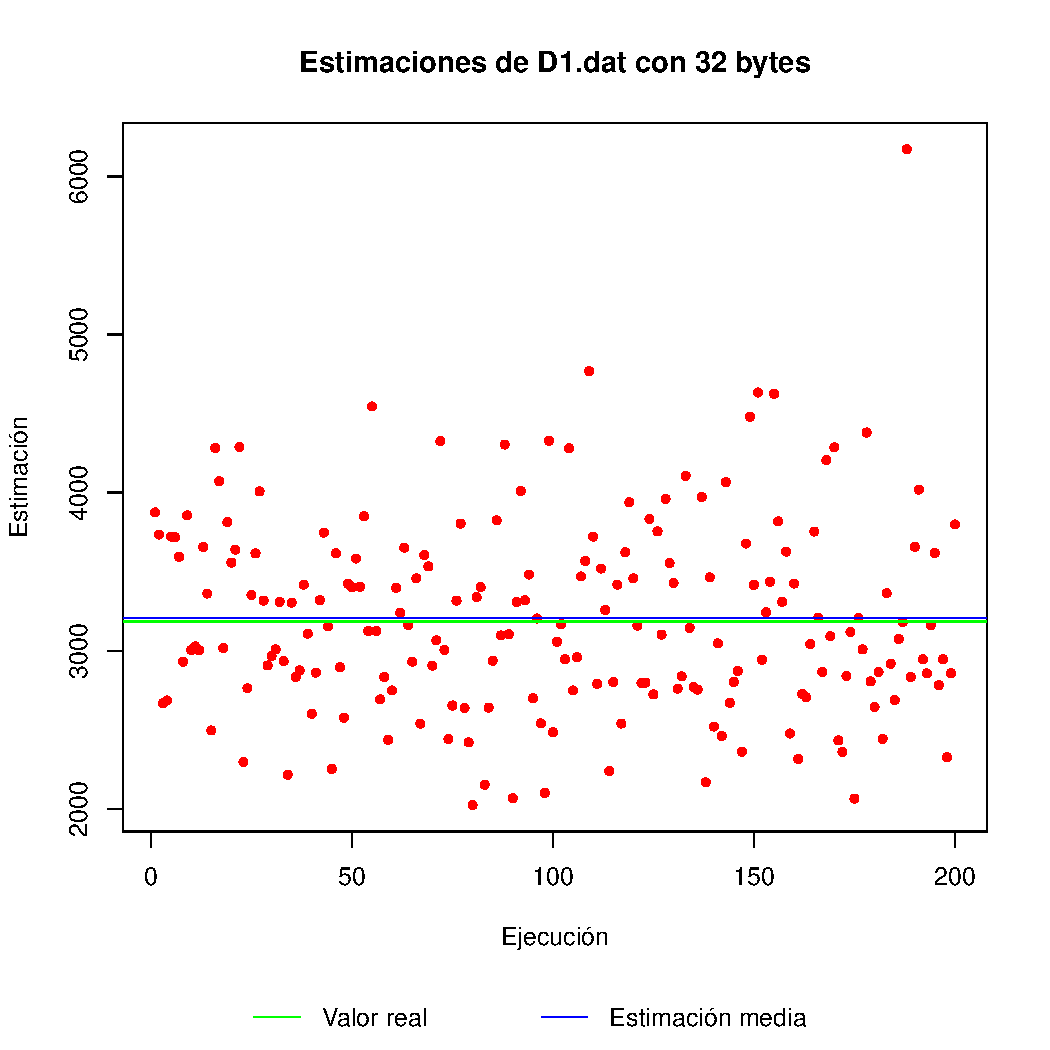
\includegraphics[width=0.64\textwidth]{../figs/D1/plot_estimation_32.pdf}
        \caption{Estimaciones en D1.dat con 32 bytes}
    \label{figura:D1_estimation_32}
\end{figure}

\begin{figure}[h!]
    \centering
        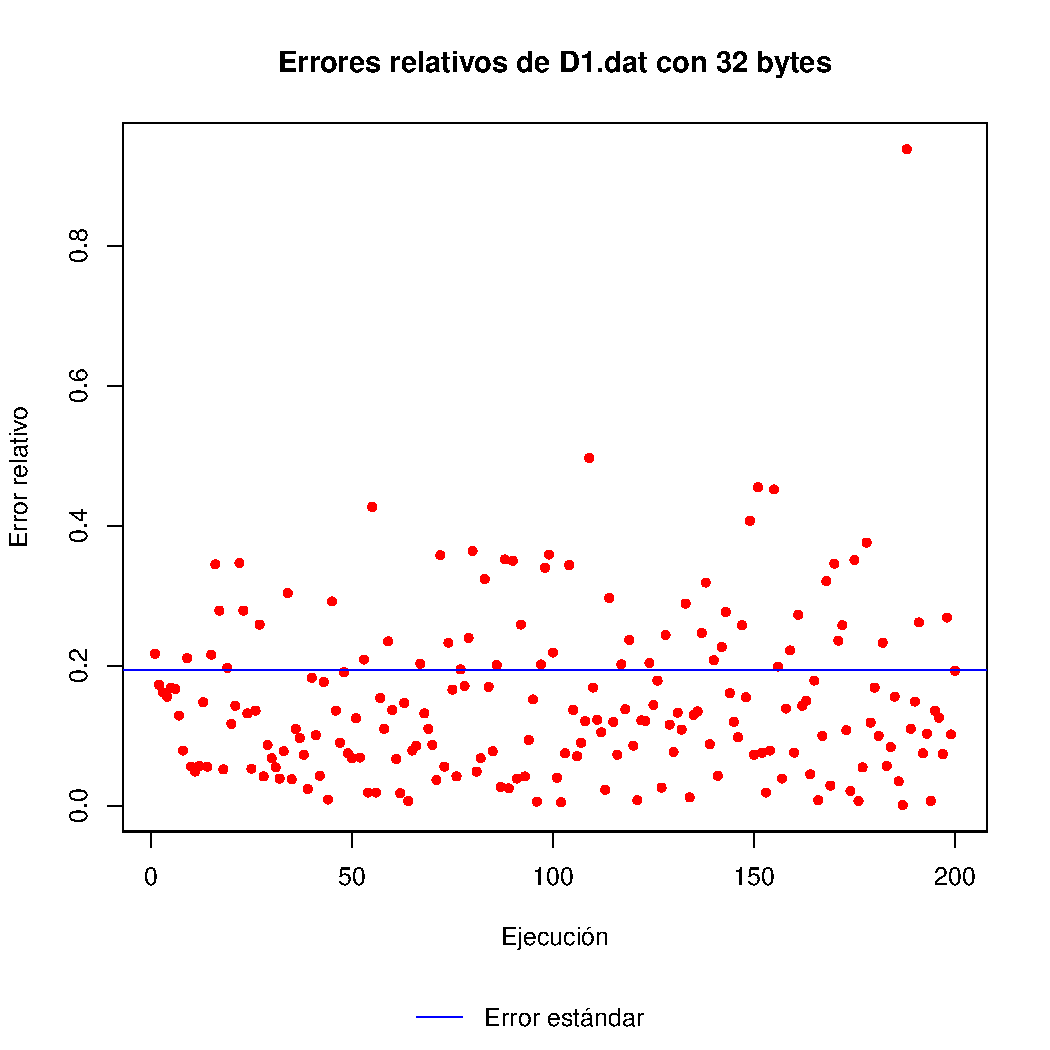
\includegraphics[width=0.64\textwidth]{../figs/D1/plot_errors_32.pdf}
        \caption{Errores relativos en D1.dat con 32 bytes}
    \label{figura:D1_errors_32}
\end{figure}

\begin{figure}[h!]
    \centering
        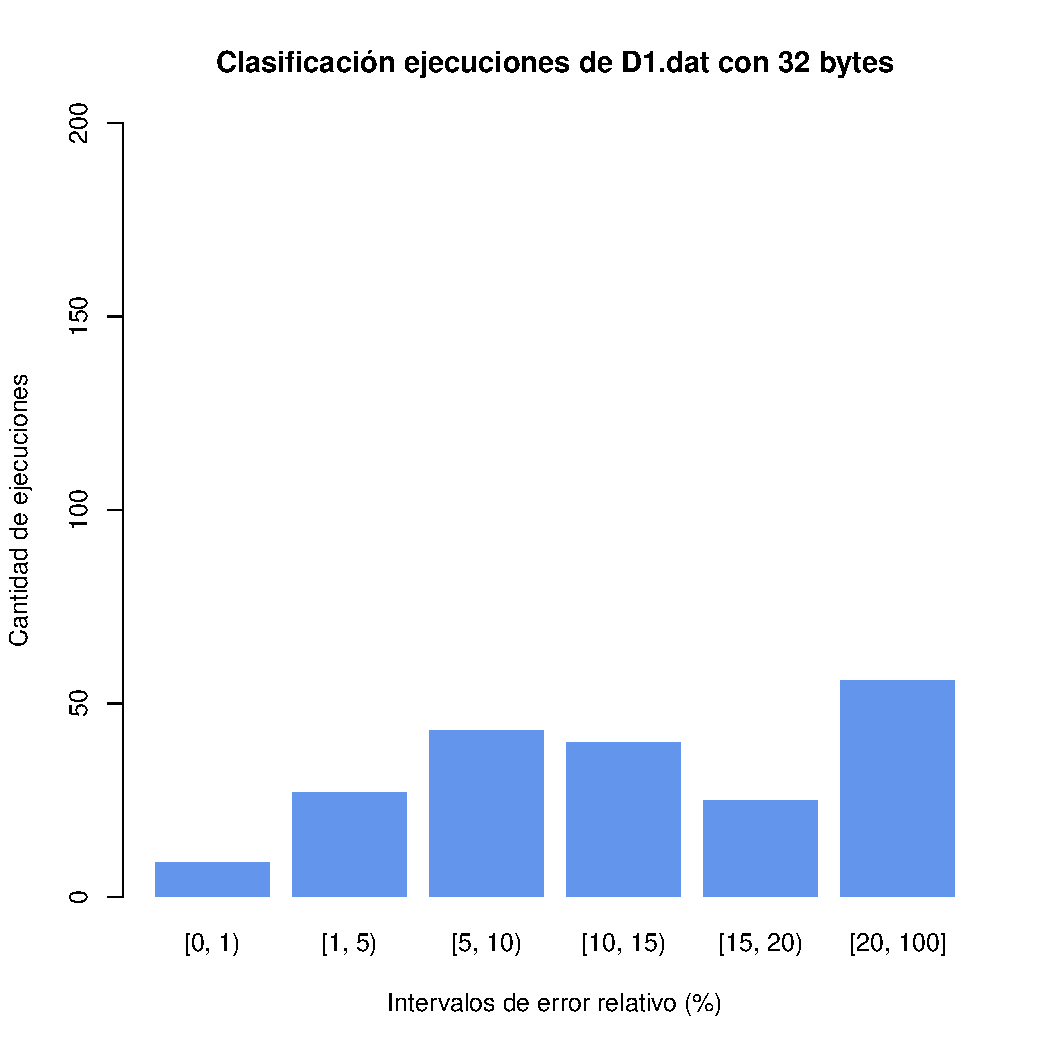
\includegraphics[width=0.64\textwidth]{../figs/D1/plot_count_32.pdf}
        \caption{Clasificación de ejecuciones en D1.dat con 32 bytes}
    \label{figura:D1_count_32}
\end{figure}

\begin{figure}[h!]
    \centering
        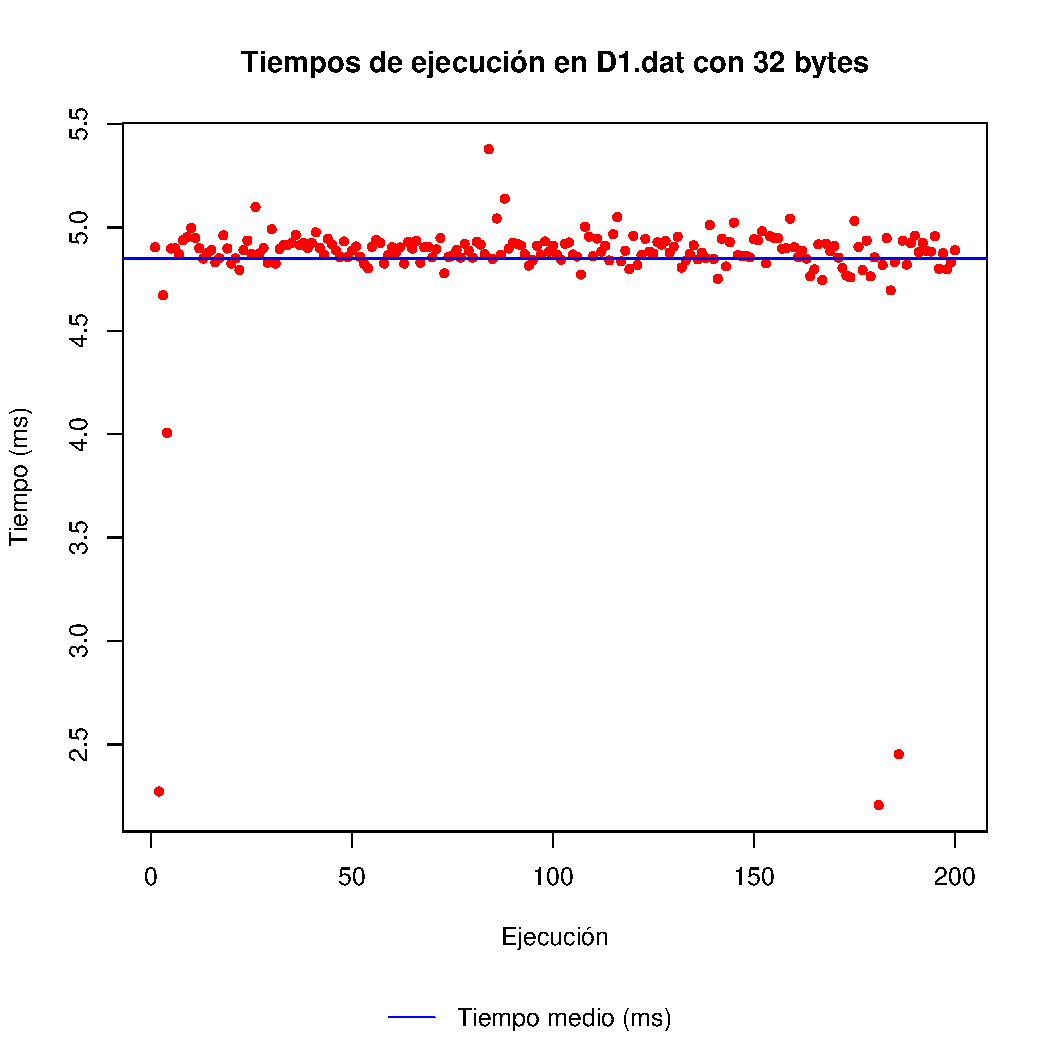
\includegraphics[width=0.64\textwidth]{../figs/D1/plot_time_32.pdf}
        \caption{Tiempos de ejecución en D1.dat con 32 bytes}
    \label{figura:D1_time_32}
\end{figure}

\clearpage
\subsubsection{64 bytes}
\begin{figure}[h!]
    \centering
        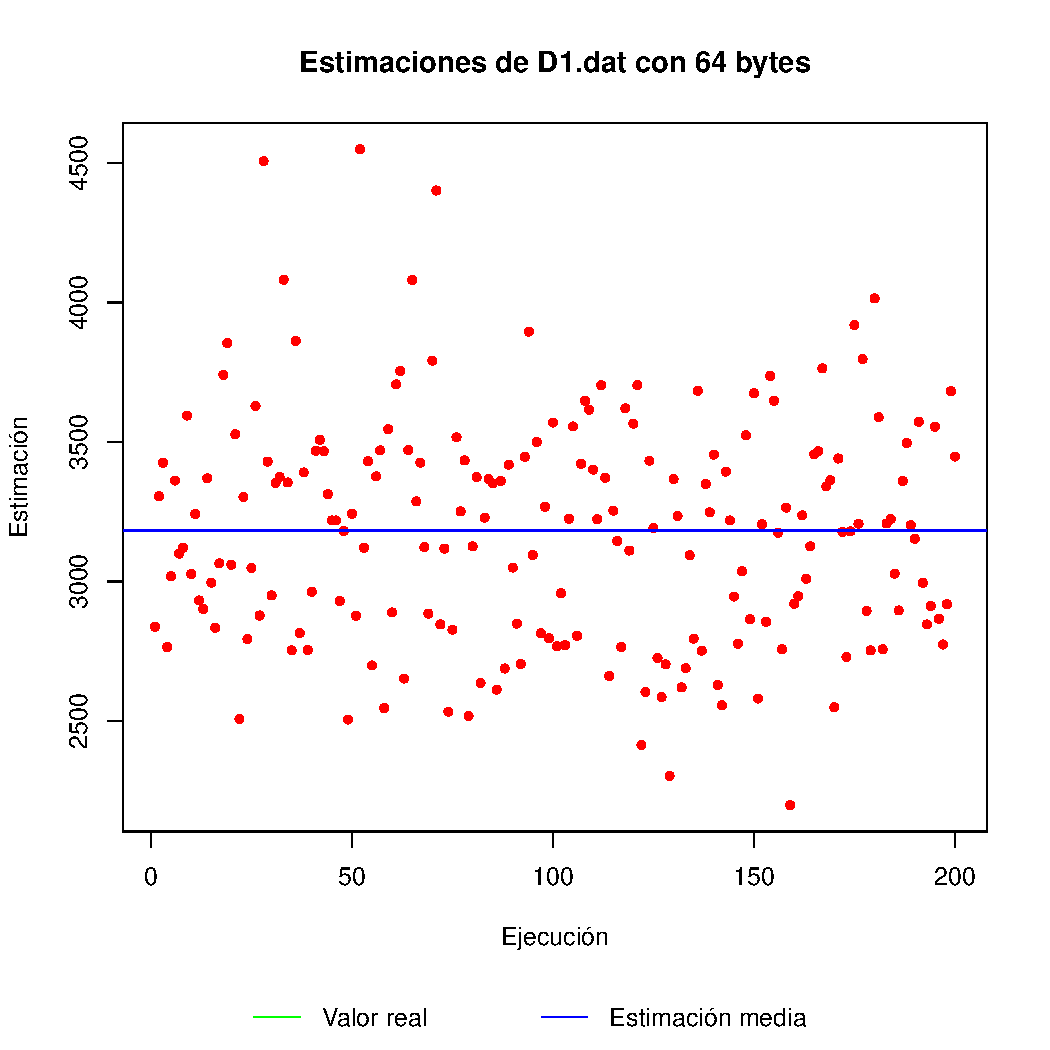
\includegraphics[width=0.64\textwidth]{../figs/D1/plot_estimation_64.pdf}
        \caption{Estimaciones en D1.dat con 64 bytes}
    \label{figura:D1_estimation_64}
\end{figure}

\begin{figure}[h!]
    \centering
        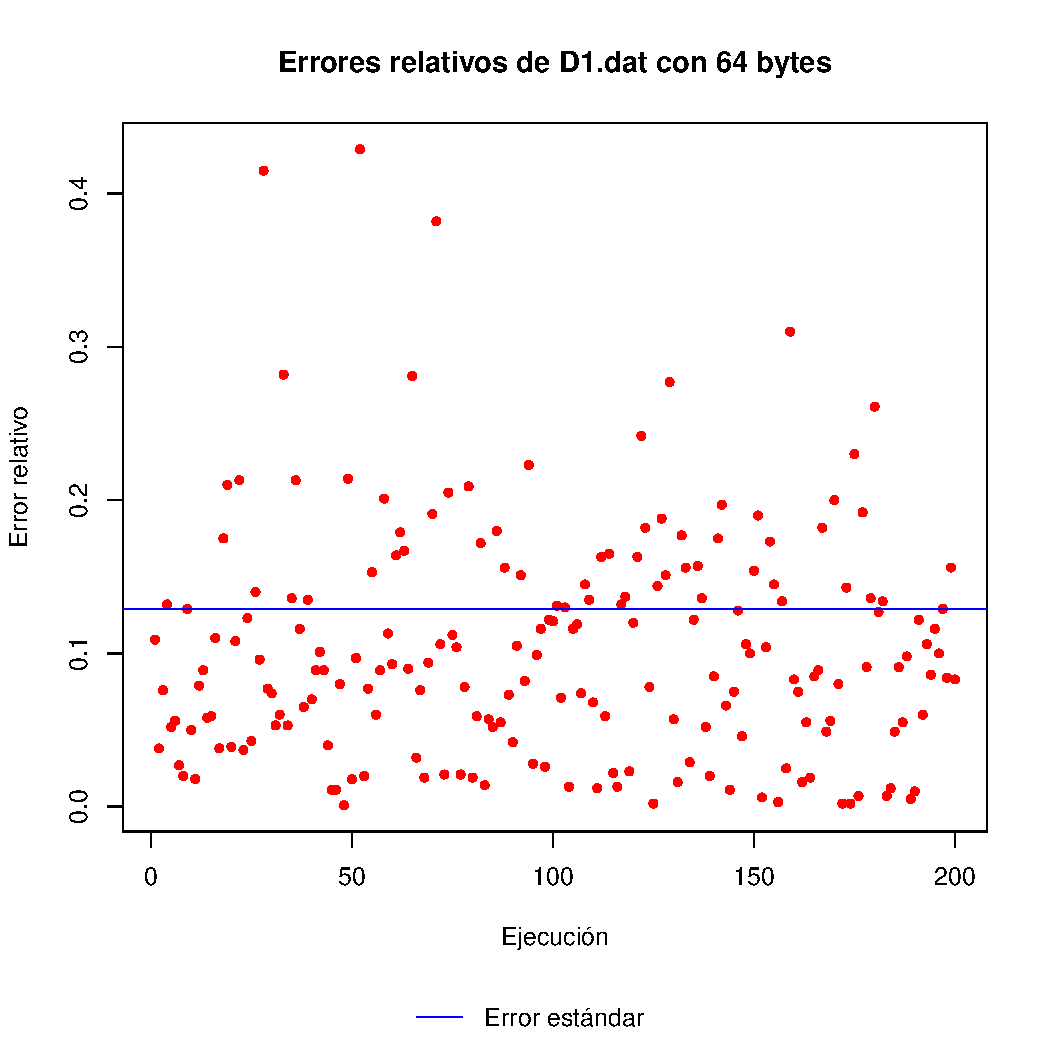
\includegraphics[width=0.64\textwidth]{../figs/D1/plot_errors_64.pdf}
        \caption{Errores relativos en D1.dat con 64 bytes}
    \label{figura:D1_errors_64}
\end{figure}

\begin{figure}[h!]
    \centering
        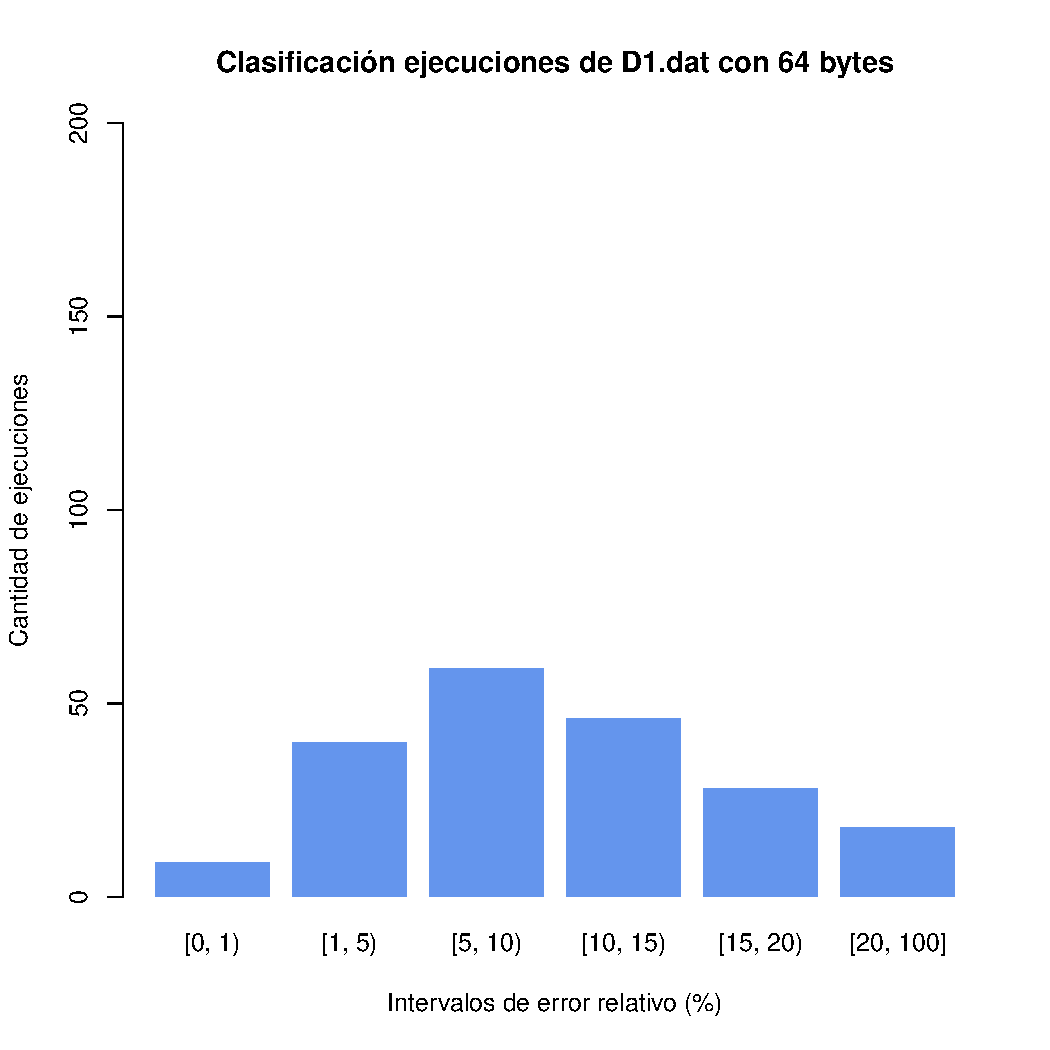
\includegraphics[width=0.64\textwidth]{../figs/D1/plot_count_64.pdf}
        \caption{Clasificación de ejecuciones en D1.dat con 64 bytes}
    \label{figura:D1_count_64}
\end{figure}

\begin{figure}[h!]
    \centering
        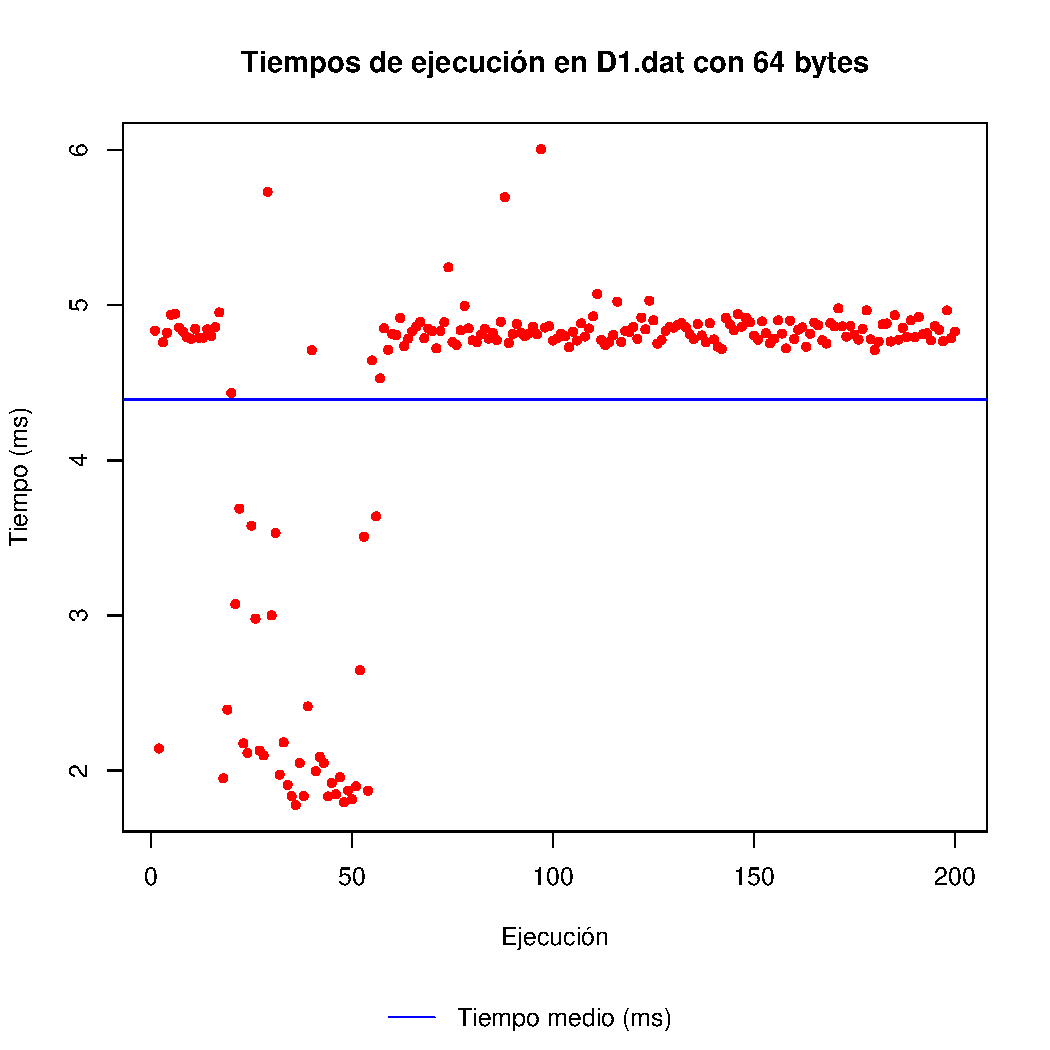
\includegraphics[width=0.64\textwidth]{../figs/D1/plot_time_64.pdf}
        \caption{Tiempos de ejecución en D1.dat con 64 bytes}
    \label{figura:D1_time_64}
\end{figure}

\clearpage
\subsubsection{128 bytes}
\begin{figure}[h!]
    \centering
        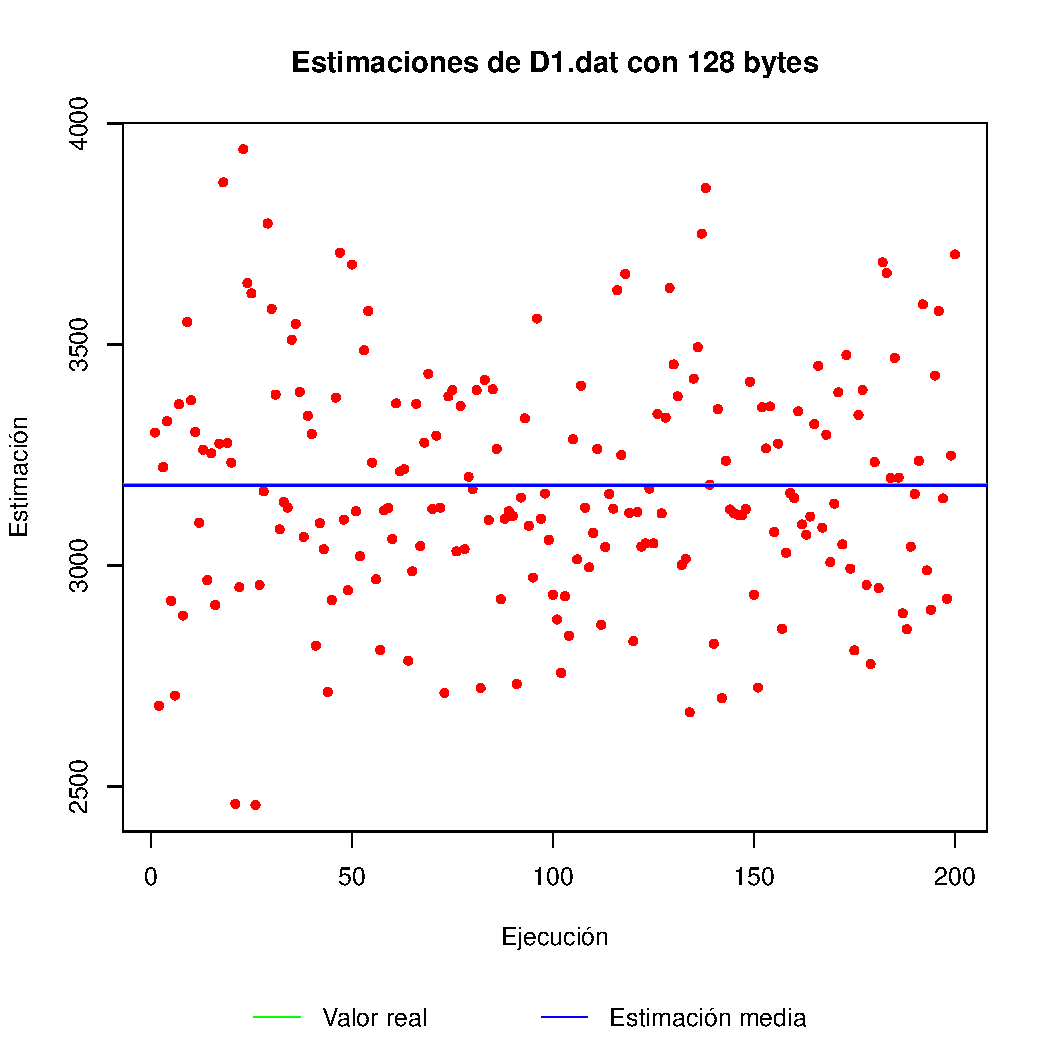
\includegraphics[width=0.64\textwidth]{../figs/D1/plot_estimation_128.pdf}
        \caption{Estimaciones en D1.dat con 128 bytes}
    \label{figura:D1_estimation_128}
\end{figure}

\begin{figure}[h!]
    \centering
        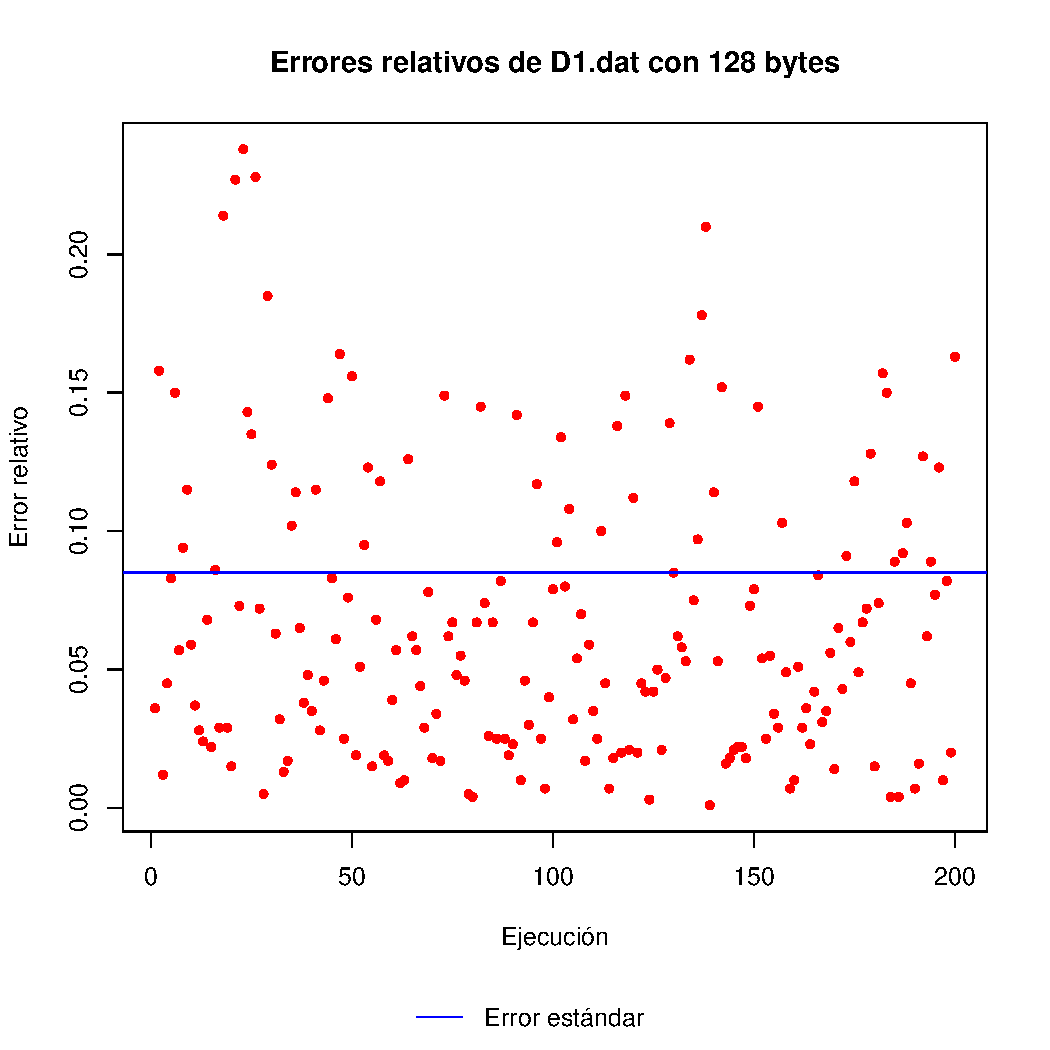
\includegraphics[width=0.64\textwidth]{../figs/D1/plot_errors_128.pdf}
        \caption{Errores relativos en D1.dat con 128 bytes}
    \label{figura:D1_errors_128}
\end{figure}

\begin{figure}[h!]
    \centering
        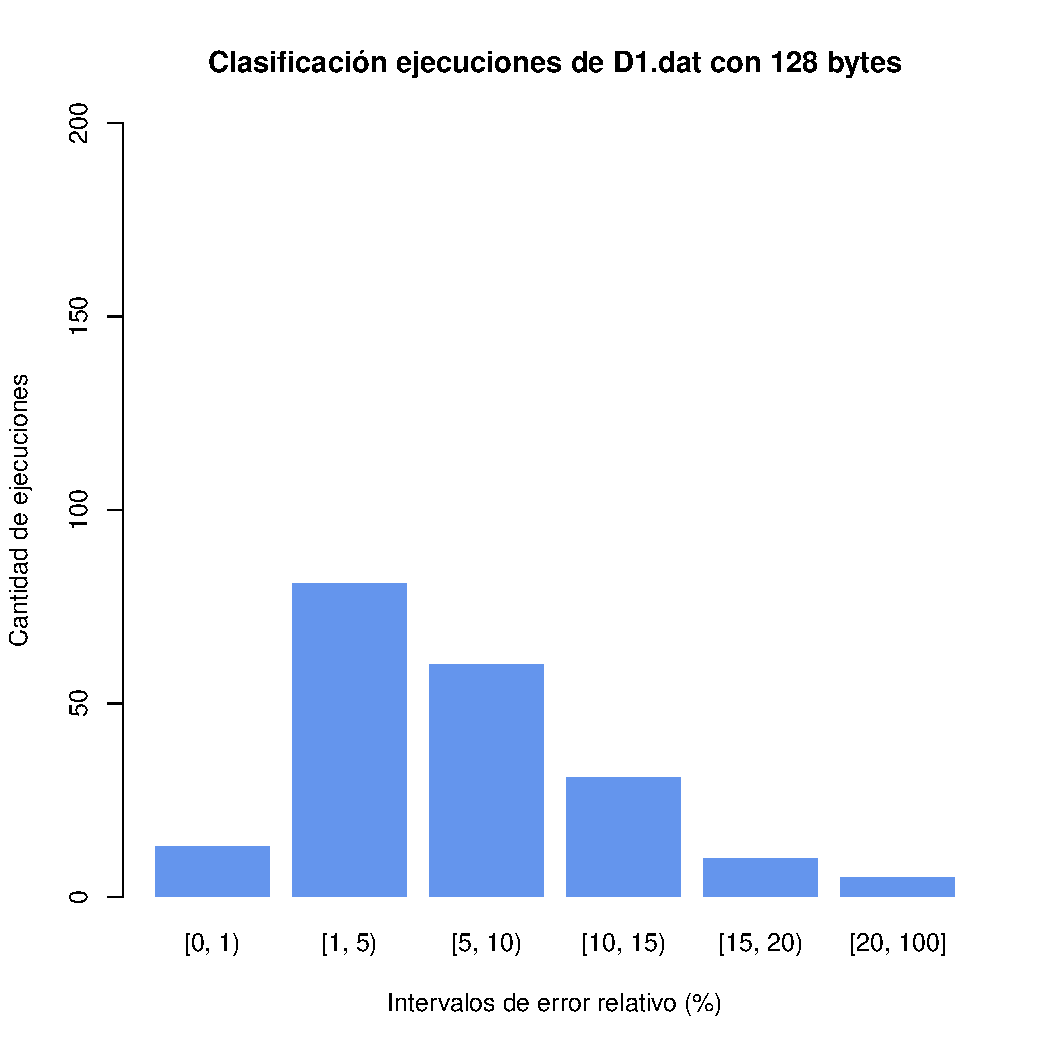
\includegraphics[width=0.64\textwidth]{../figs/D1/plot_count_128.pdf}
        \caption{Clasificación de ejecuciones en D1.dat con 128 bytes}
    \label{figura:D1_count_128}
\end{figure}

\begin{figure}[h!]
    \centering
        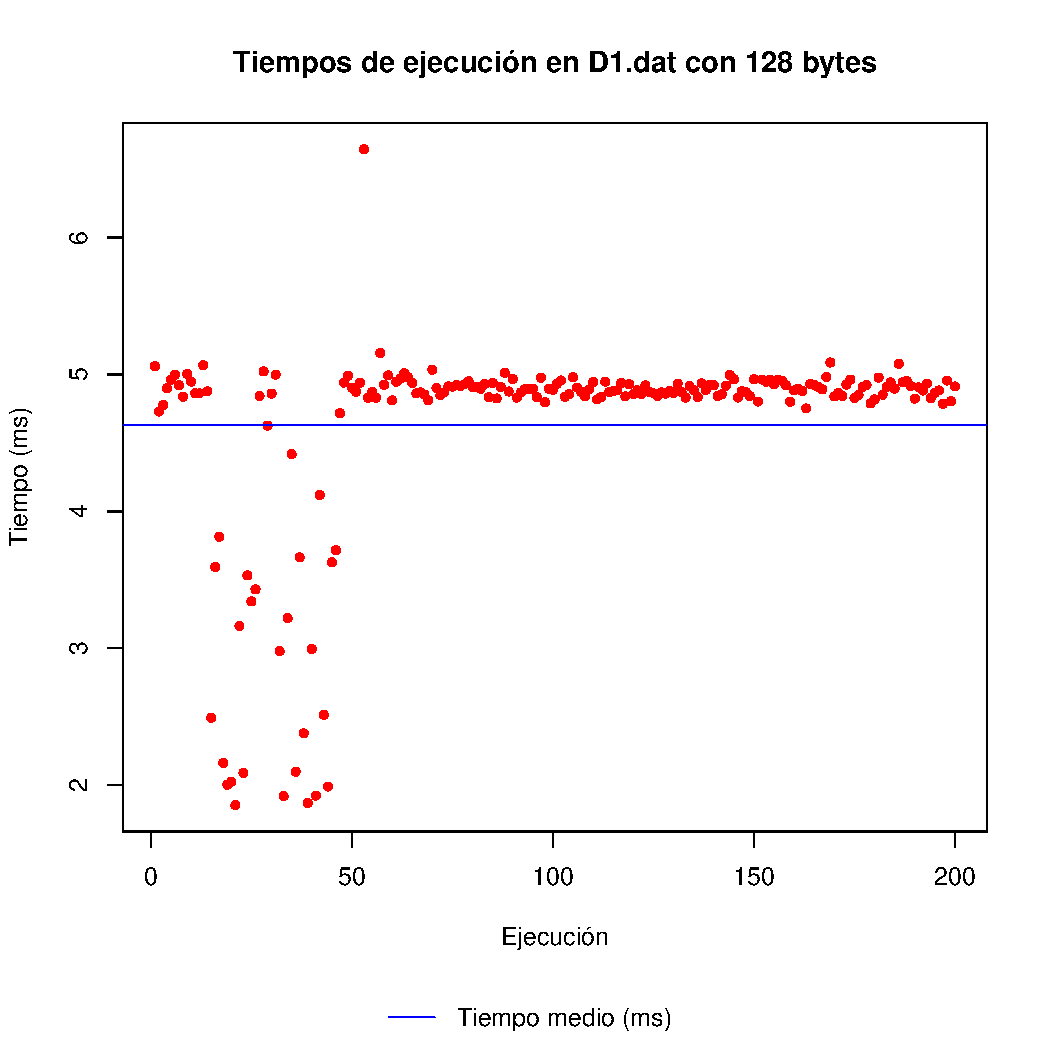
\includegraphics[width=0.64\textwidth]{../figs/D1/plot_time_128.pdf}
        \caption{Tiempos de ejecución en D1.dat con 128 bytes}
    \label{figura:D1_time_128}
\end{figure}

\clearpage
\subsubsection{256 bytes}
\begin{figure}[h!]
    \centering
        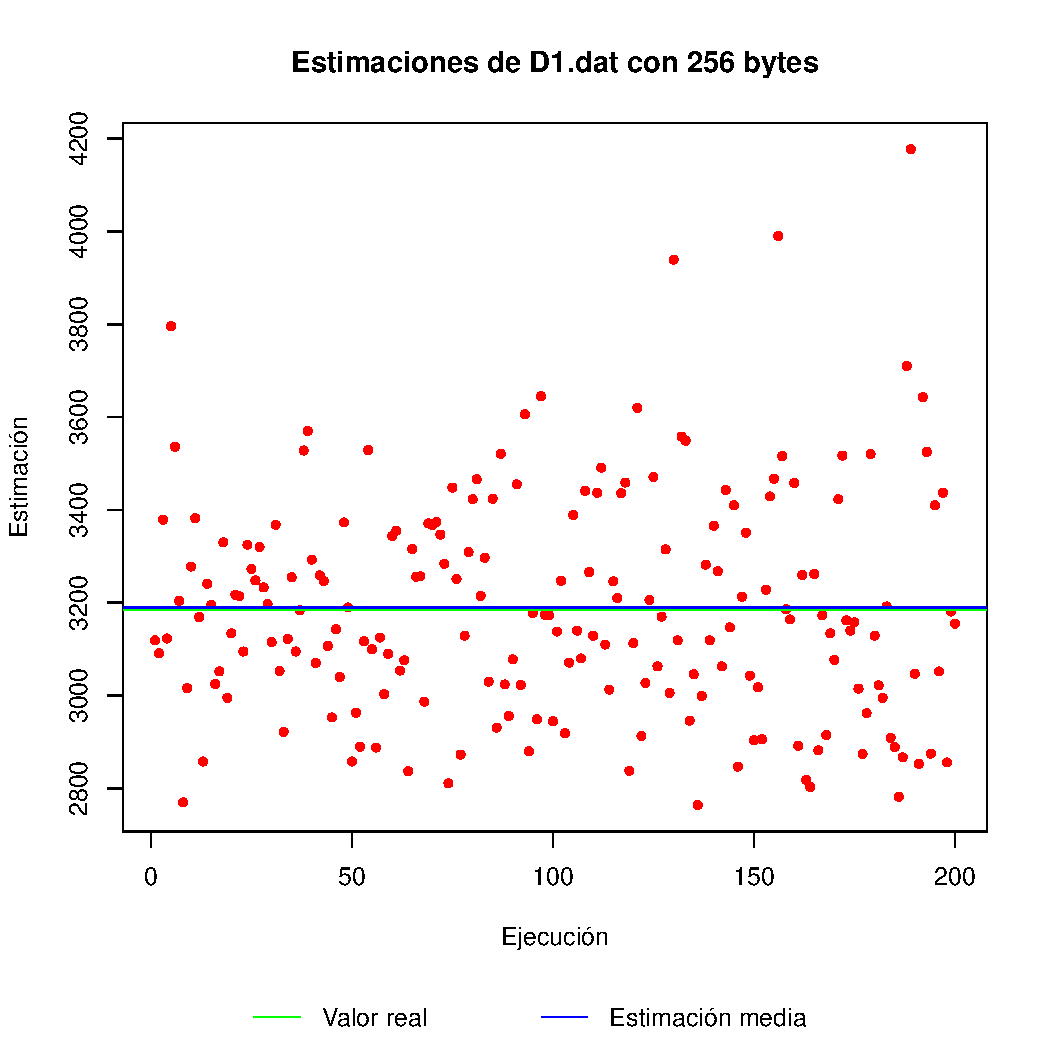
\includegraphics[width=0.64\textwidth]{../figs/D1/plot_estimation_256.pdf}
        \caption{Estimaciones en D1.dat con 256 bytes}
    \label{figura:D1_estimation_256}
\end{figure}

\begin{figure}[h!]
    \centering
        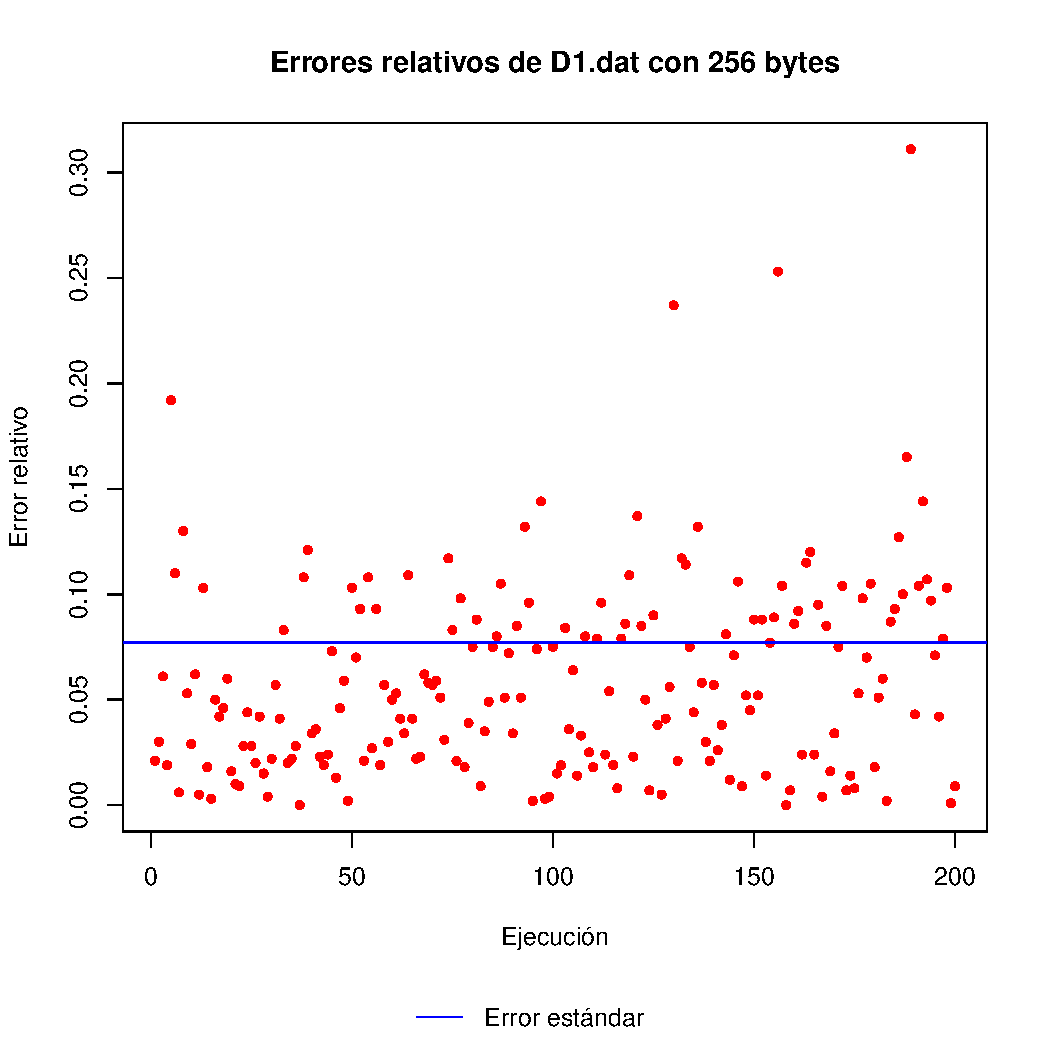
\includegraphics[width=0.64\textwidth]{../figs/D1/plot_errors_256.pdf}
        \caption{Errores relativos en D1.dat con 256 bytes}
    \label{figura:D1_errors_256}
\end{figure}

\begin{figure}[h!]
    \centering
        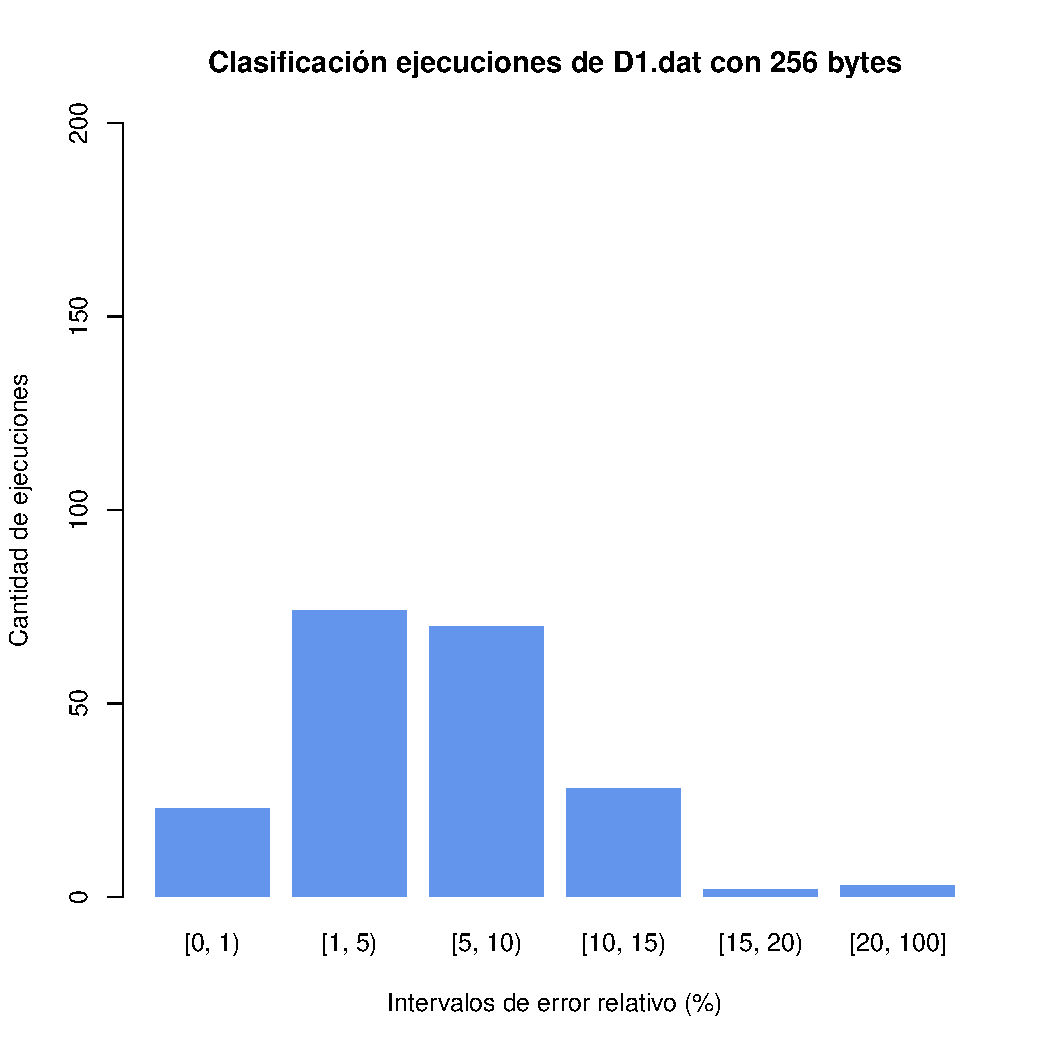
\includegraphics[width=0.64\textwidth]{../figs/D1/plot_count_256.pdf}
        \caption{Clasificación de ejecuciones en D1.dat con 256 bytes}
    \label{figura:D1_count_256}
\end{figure}

\begin{figure}[h!]
    \centering
        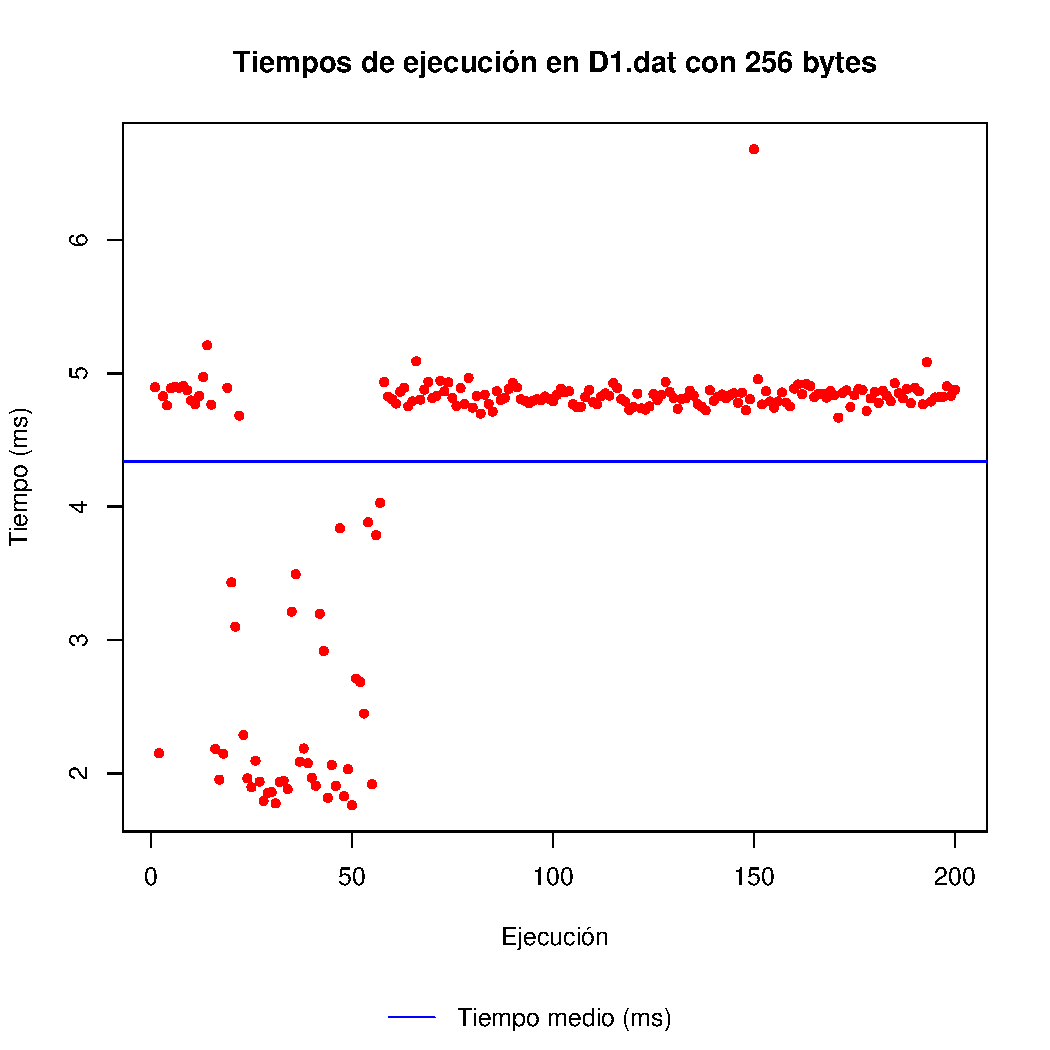
\includegraphics[width=0.64\textwidth]{../figs/D1/plot_time_256.pdf}
        \caption{Tiempos de ejecución en D1.dat con 256 bytes}
    \label{figura:D1_time_256}
\end{figure}

\clearpage
\subsubsection{512 bytes}
\begin{figure}[h!]
    \centering
        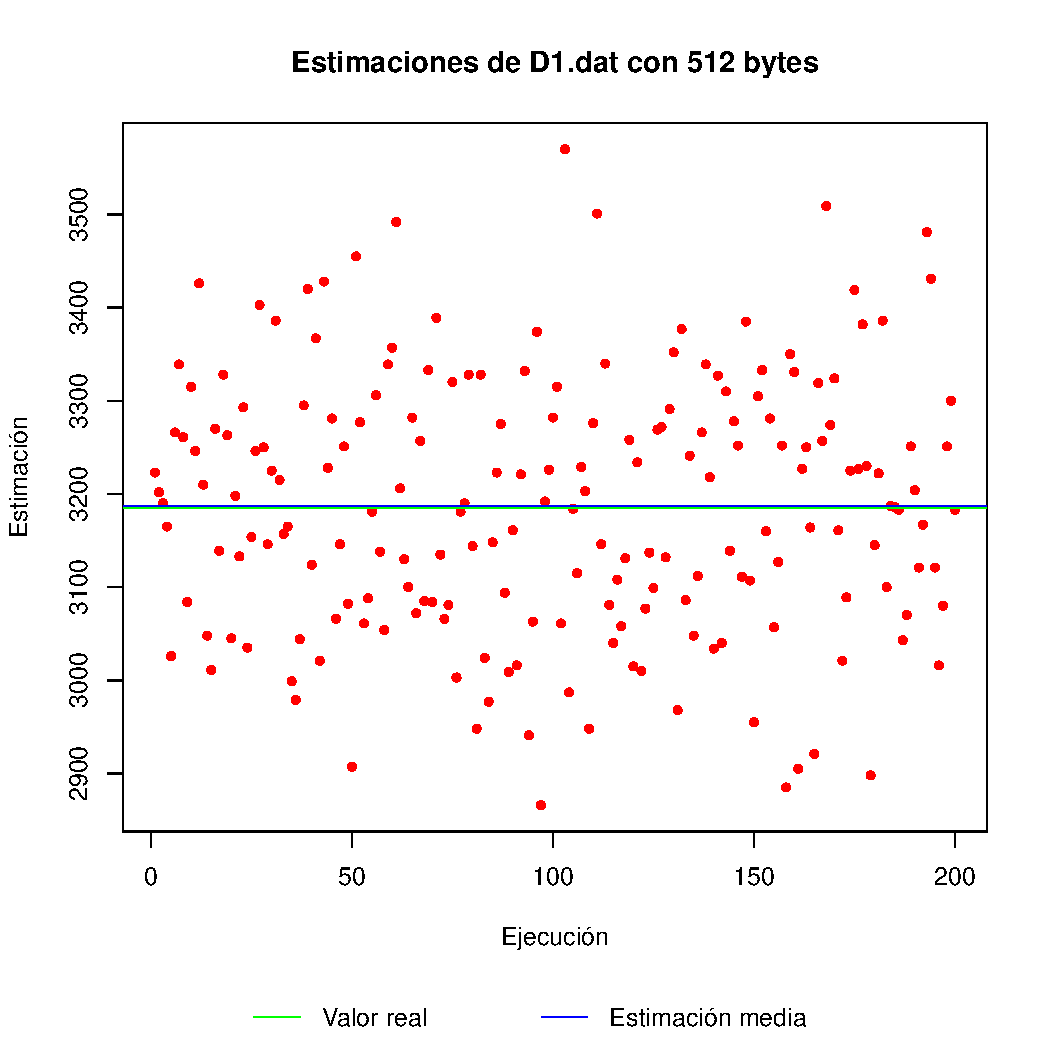
\includegraphics[width=0.64\textwidth]{../figs/D1/plot_estimation_512.pdf}
        \caption{Estimaciones en D1.dat con 512 bytes}
    \label{figura:D1_estimation_512}
\end{figure}

\begin{figure}[h!]
    \centering
        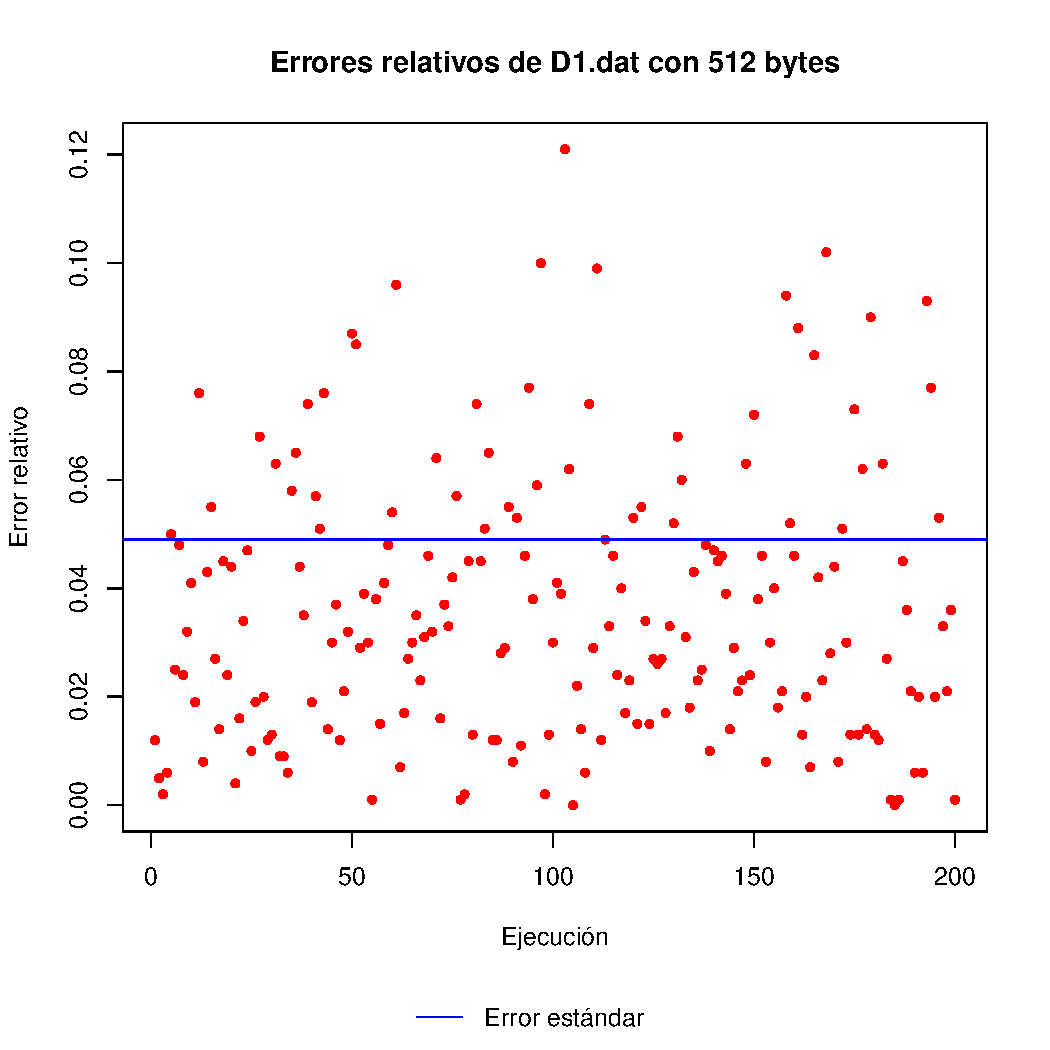
\includegraphics[width=0.64\textwidth]{../figs/D1/plot_errors_512.pdf}
        \caption{Errores relativos en D1.dat con 512 bytes}
    \label{figura:D1_errors_512}
\end{figure}

\begin{figure}[h!]
    \centering
        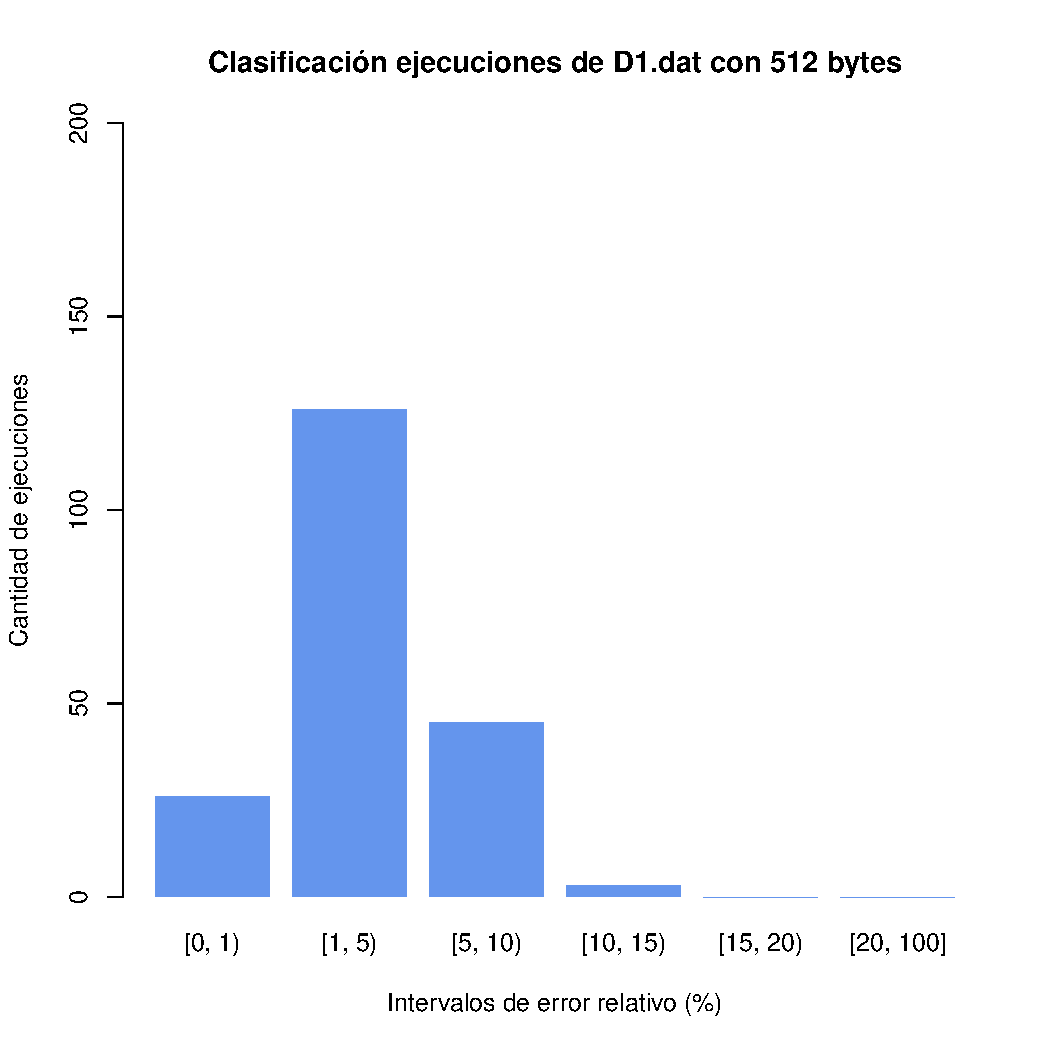
\includegraphics[width=0.64\textwidth]{../figs/D1/plot_count_512.pdf}
        \caption{Clasificación de ejecuciones en D1.dat con 512 bytes}
    \label{figura:D1_count_512}
\end{figure}

\begin{figure}[h!]
    \centering
        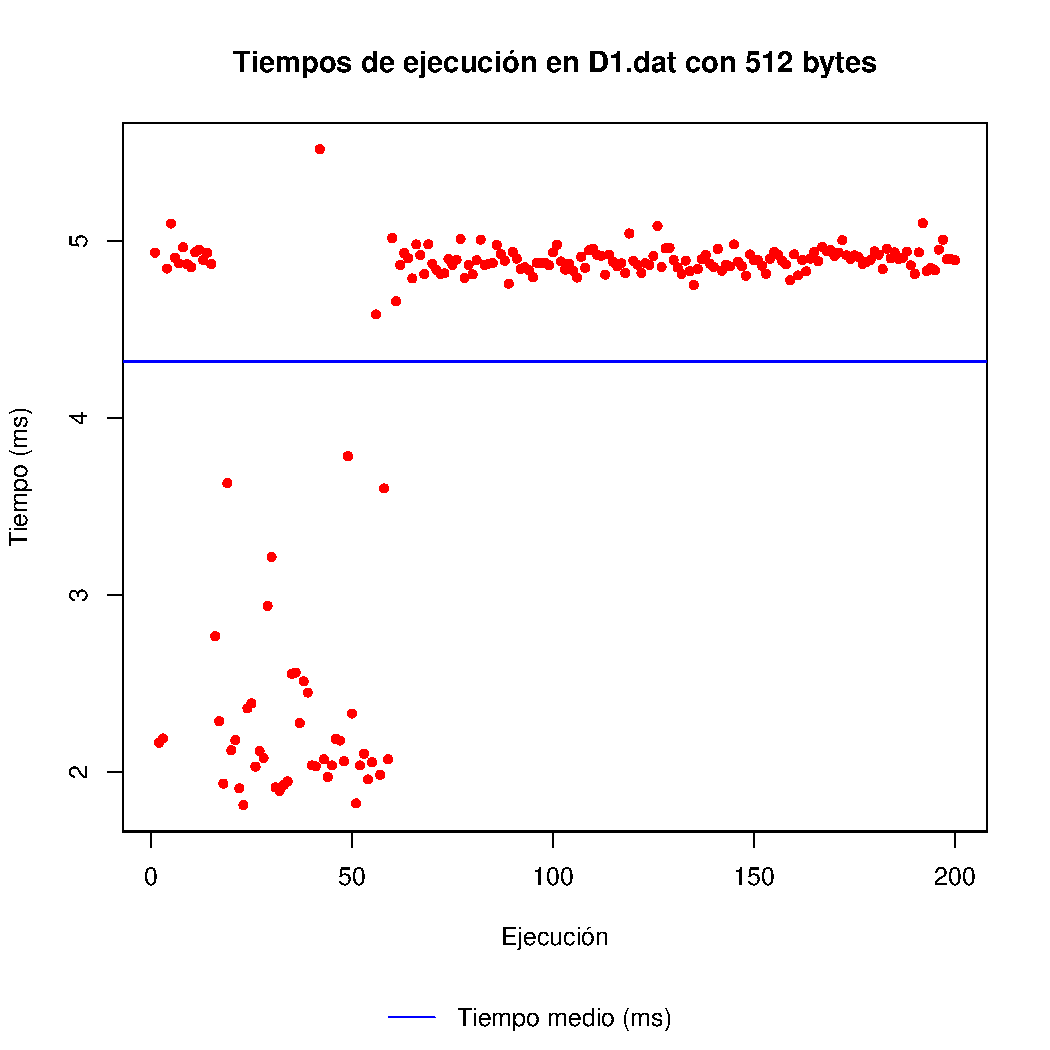
\includegraphics[width=0.64\textwidth]{../figs/D1/plot_time_512.pdf}
        \caption{Tiempos de ejecución en D1.dat con 512 bytes}
    \label{figura:D1_time_512}
\end{figure}

\clearpage
\subsubsection{1024 bytes}
\begin{figure}[h!]
    \centering
        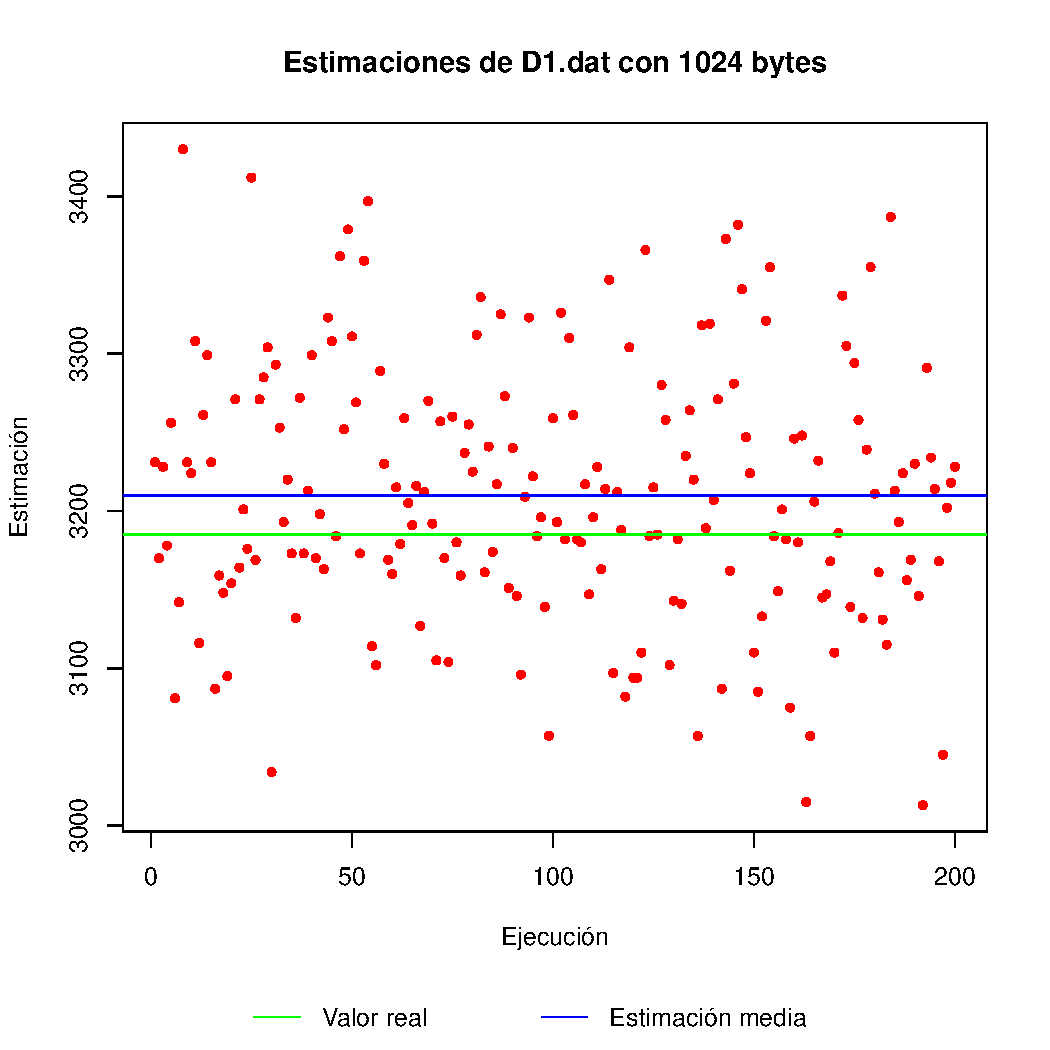
\includegraphics[width=0.64\textwidth]{../figs/D1/plot_estimation_1024.pdf}
        \caption{Estimaciones en D1.dat con 1024 bytes}
    \label{figura:D1_estimation_1024}
\end{figure}

\begin{figure}[h!]
    \centering
        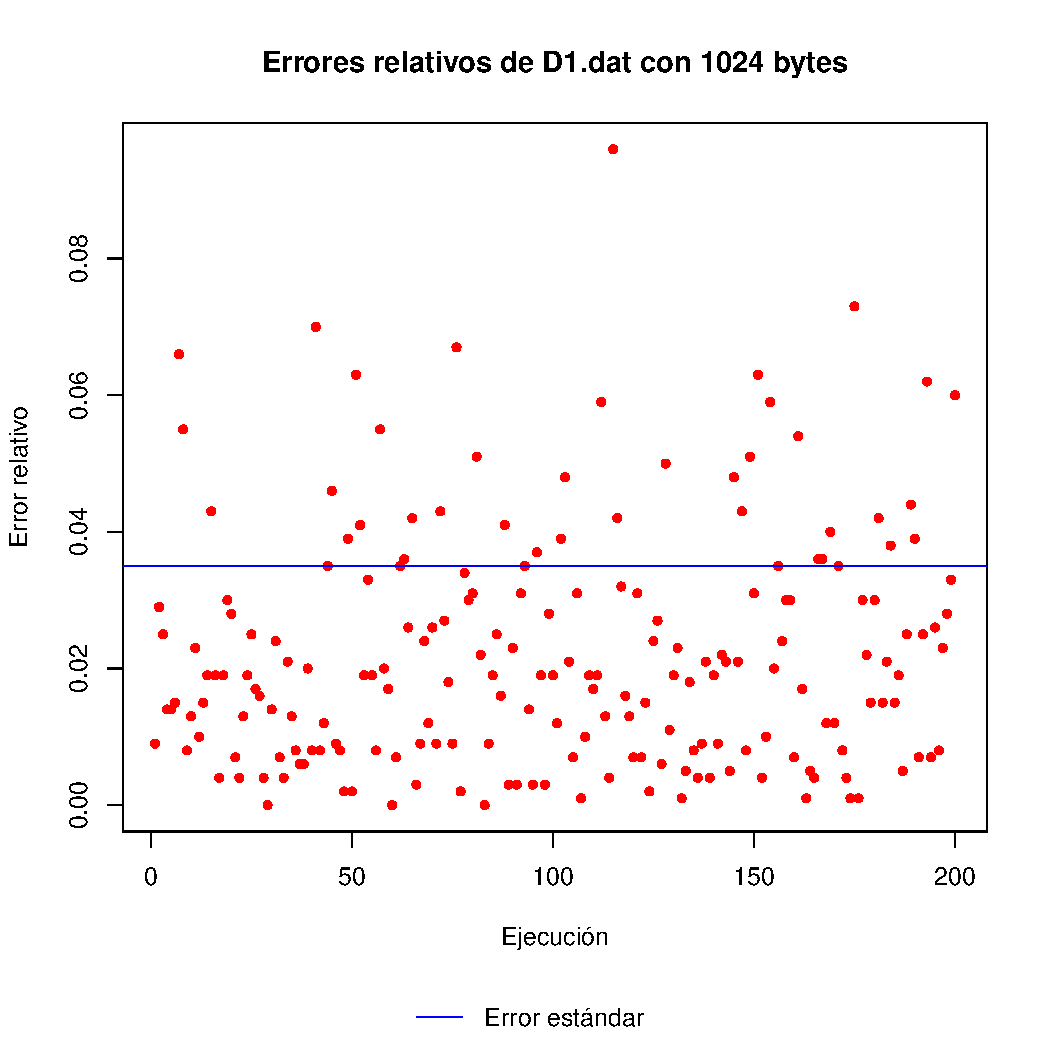
\includegraphics[width=0.64\textwidth]{../figs/D1/plot_errors_1024.pdf}
        \caption{Errores relativos en D1.dat con 1024 bytes}
    \label{figura:D1_errors_1024}
\end{figure}

\begin{figure}[h!]
    \centering
        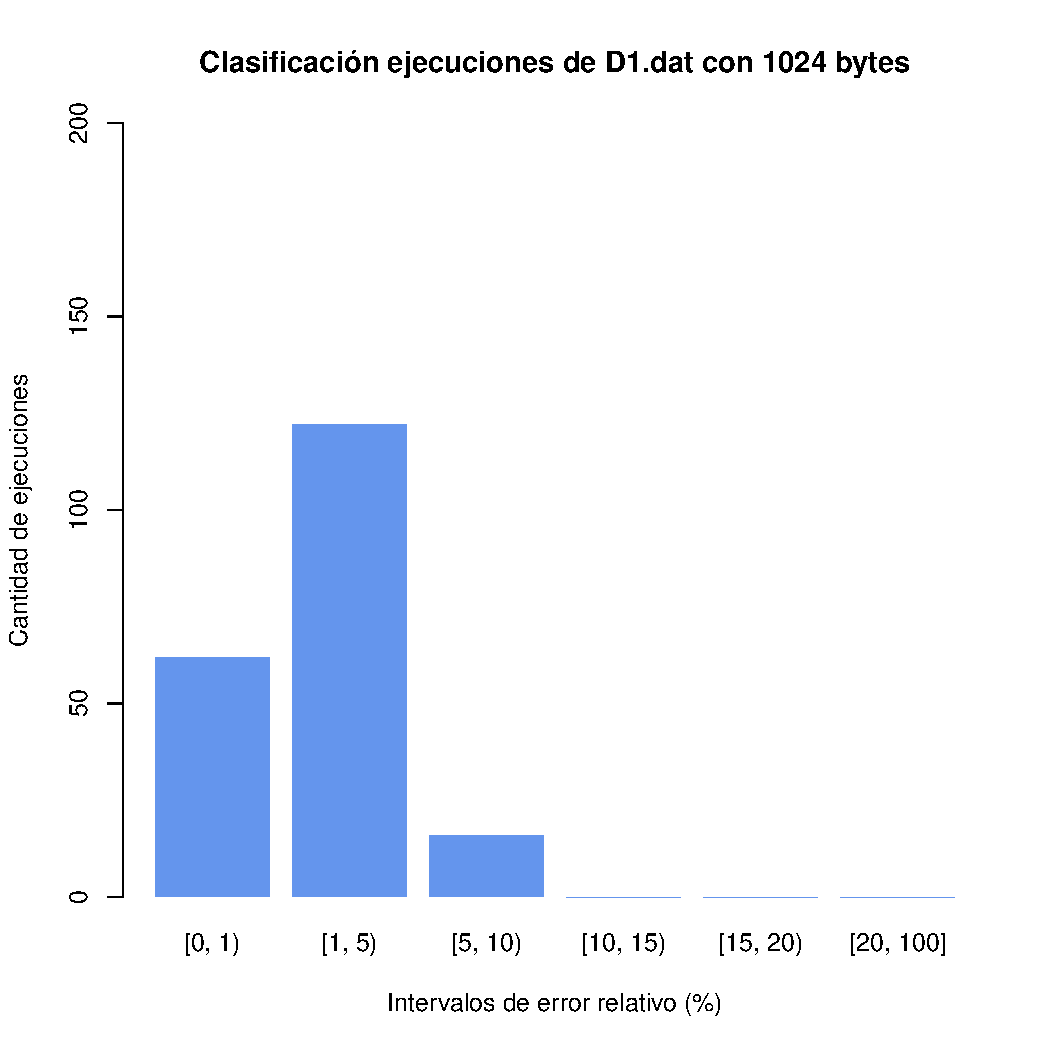
\includegraphics[width=0.64\textwidth]{../figs/D1/plot_count_1024.pdf}
        \caption{Clasificación de ejecuciones en D1.dat con 1024 bytes}
    \label{figura:D1_count_1024}
\end{figure}

\begin{figure}[h!]
    \centering
        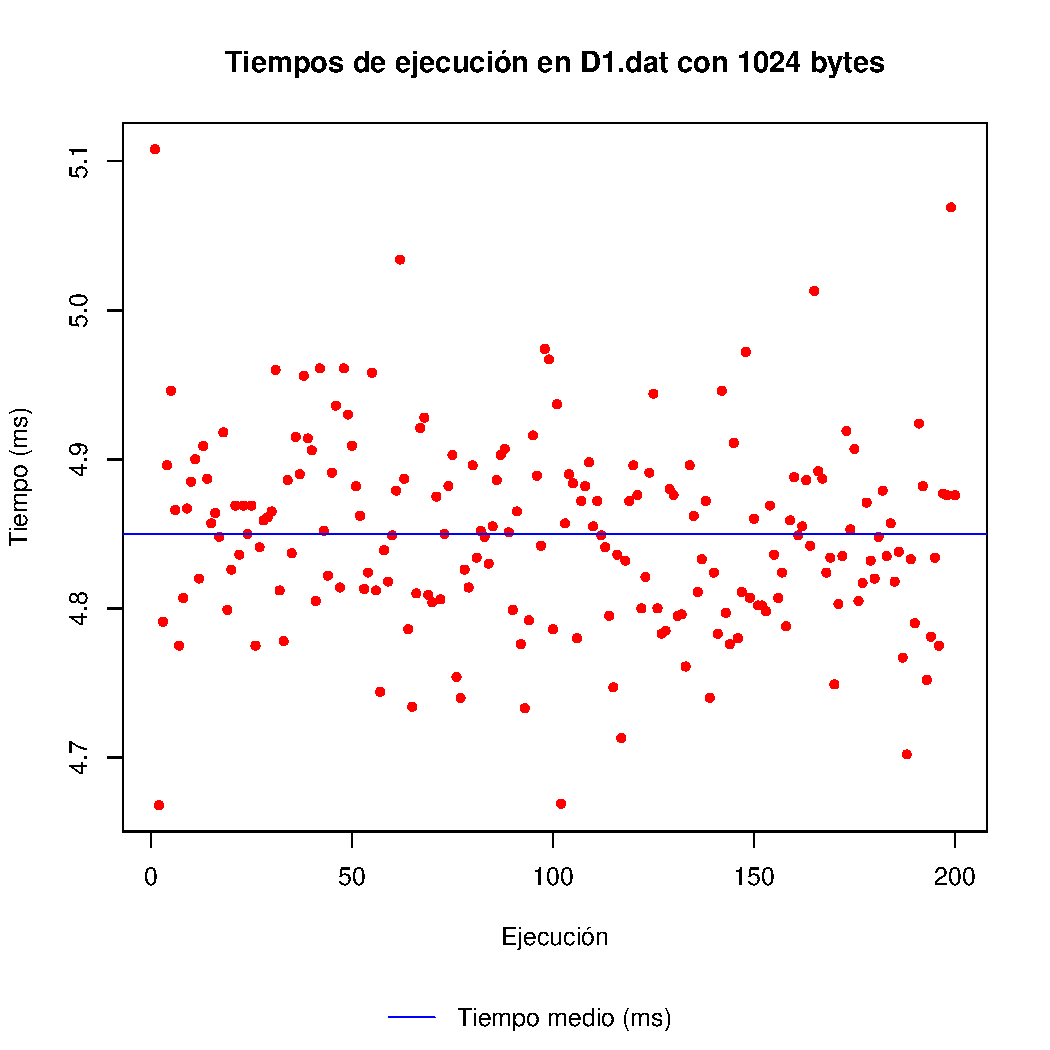
\includegraphics[width=0.64\textwidth]{../figs/D1/plot_time_1024.pdf}
        \caption{Tiempos de ejecución en D1.dat con 1024 bytes}
    \label{figura:D1_time_1024}
\end{figure}

\clearpage
\subsubsection{2048 bytes}
\begin{figure}[h!]
    \centering
        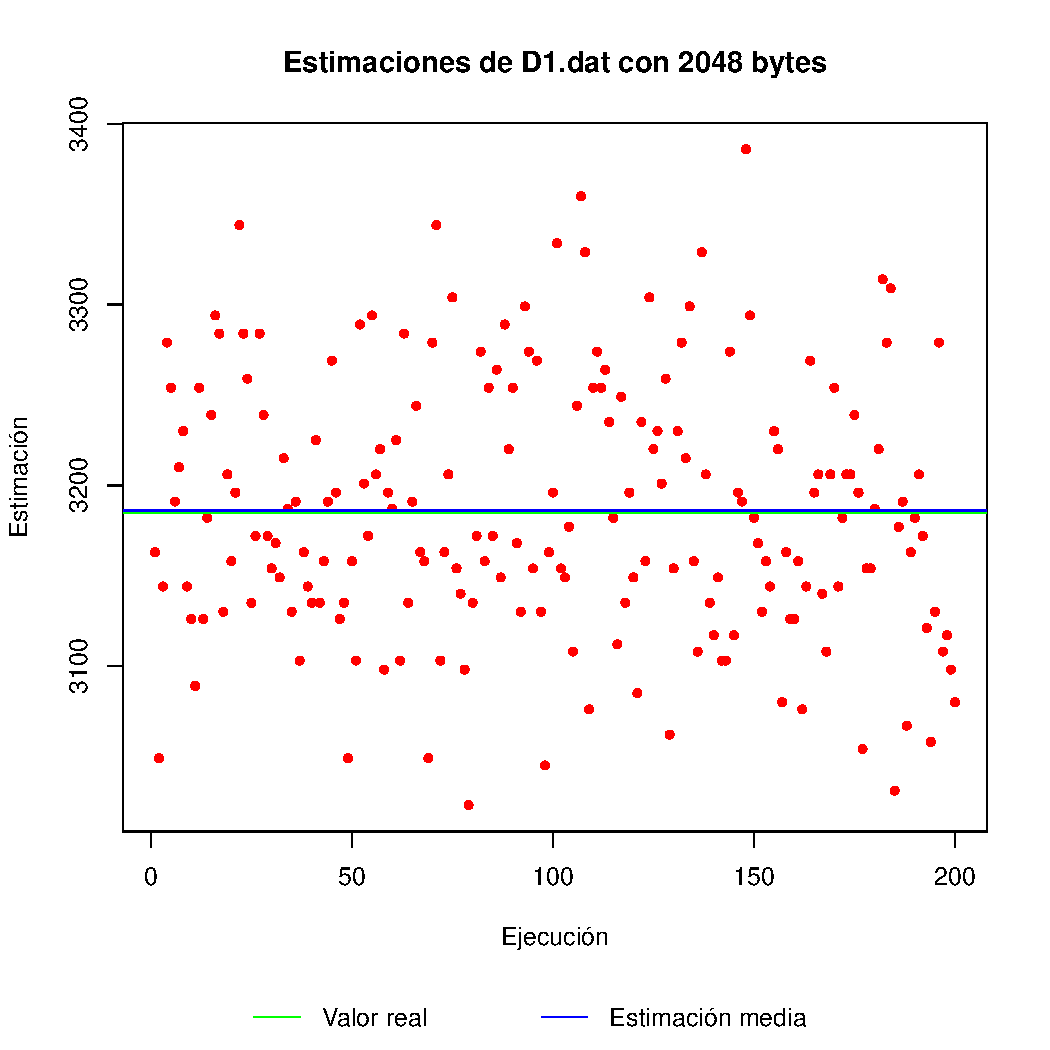
\includegraphics[width=0.64\textwidth]{../figs/D1/plot_estimation_2048.pdf}
        \caption{Estimaciones en D1.dat con 2048 bytes}
    \label{figura:D1_estimation_2048}
\end{figure}

\begin{figure}[h!]
    \centering
        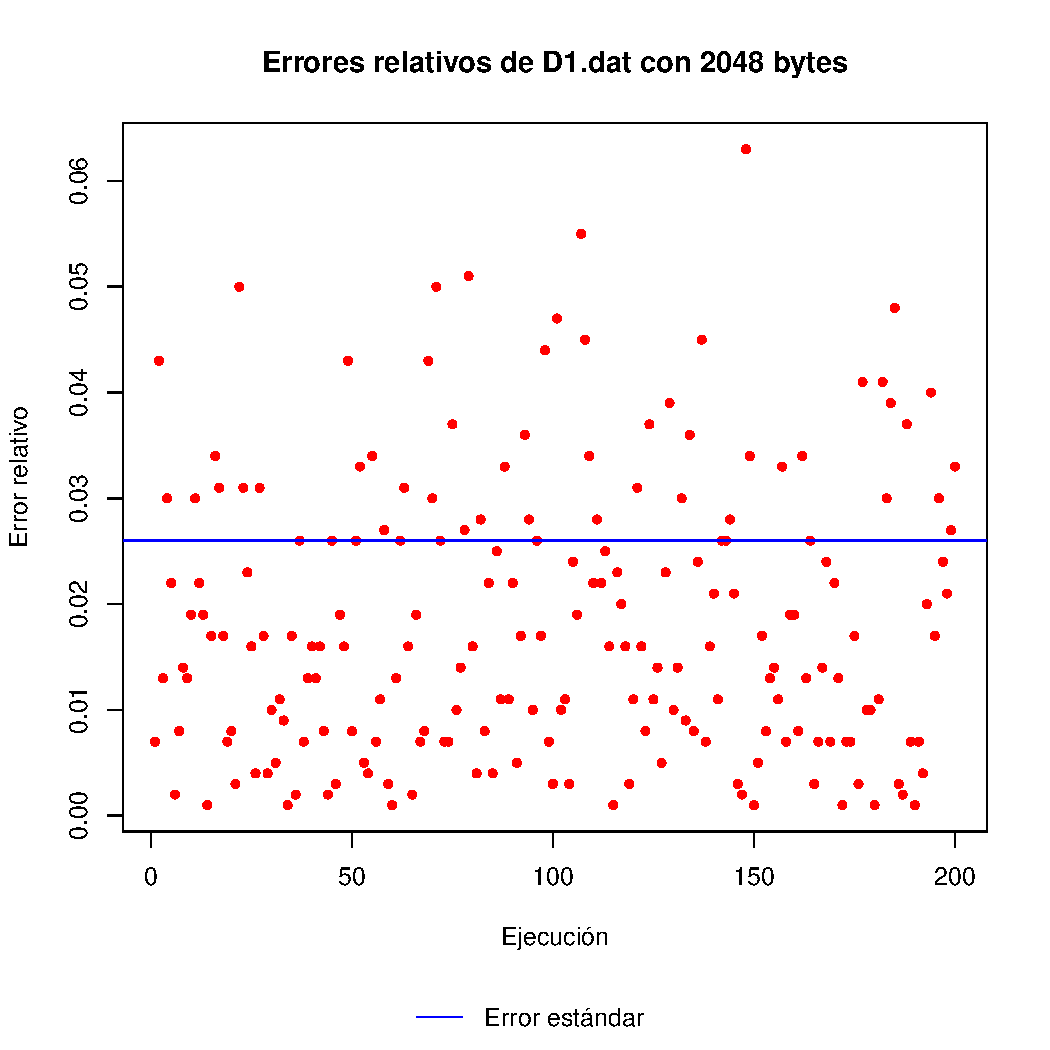
\includegraphics[width=0.64\textwidth]{../figs/D1/plot_errors_2048.pdf}
        \caption{Errores relativos en D1.dat con 2048 bytes}
    \label{figura:D1_errors_2048}
\end{figure}

\begin{figure}[h!]
    \centering
        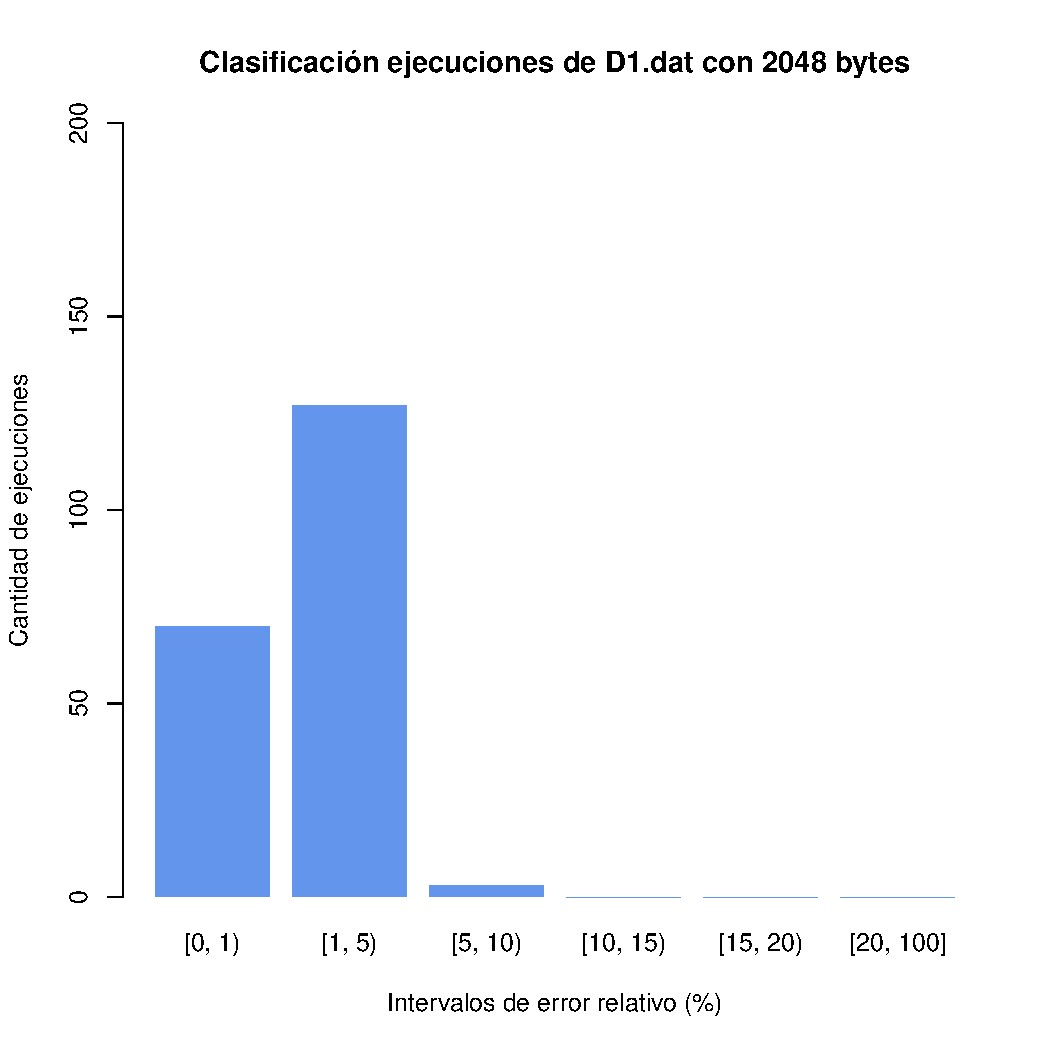
\includegraphics[width=0.64\textwidth]{../figs/D1/plot_count_2048.pdf}
        \caption{Clasificación de ejecuciones en D1.dat con 2048 bytes}
    \label{figura:D1_count_2048}
\end{figure}

\begin{figure}[h!]
    \centering
        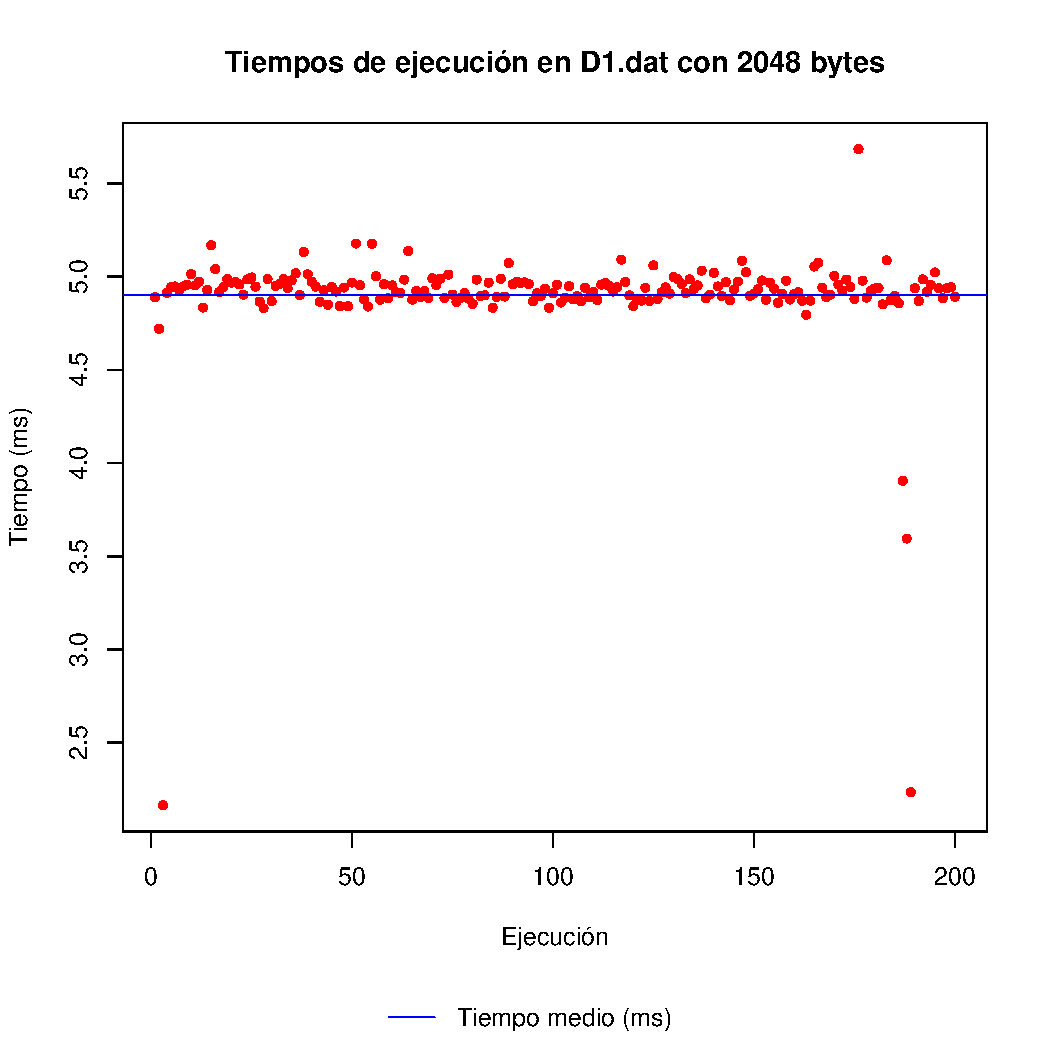
\includegraphics[width=0.64\textwidth]{../figs/D1/plot_time_2048.pdf}
        \caption{Tiempos de ejecución en D1.dat con 2048 bytes}
    \label{figura:D1_time_2048}
\end{figure}

\clearpage
\subsubsection{4096 bytes}
\begin{figure}[h!]
    \centering
        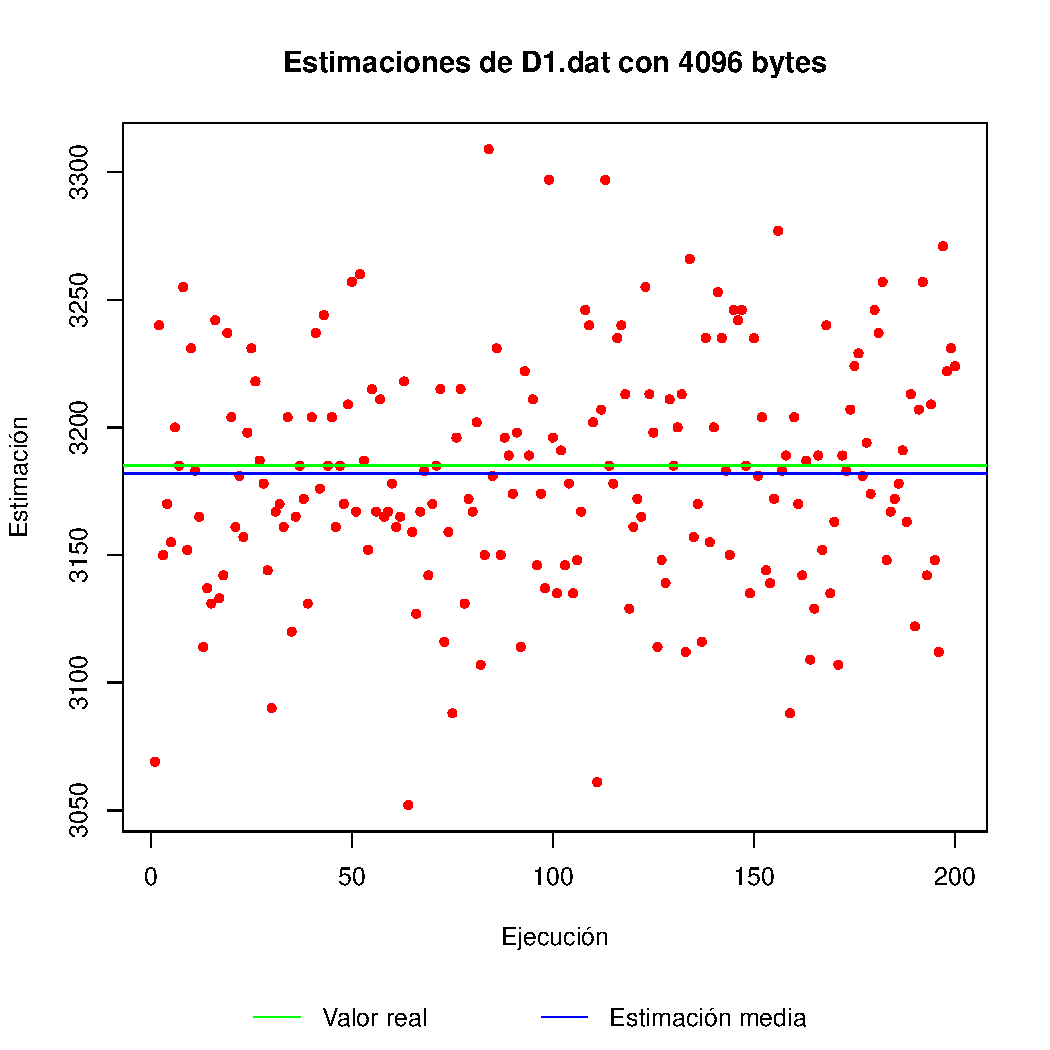
\includegraphics[width=0.64\textwidth]{../figs/D1/plot_estimation_4096.pdf}
        \caption{Estimaciones en D1.dat con 4096 bytes}
    \label{figura:D1_estimation_4096}
\end{figure}

\begin{figure}[h!]
    \centering
        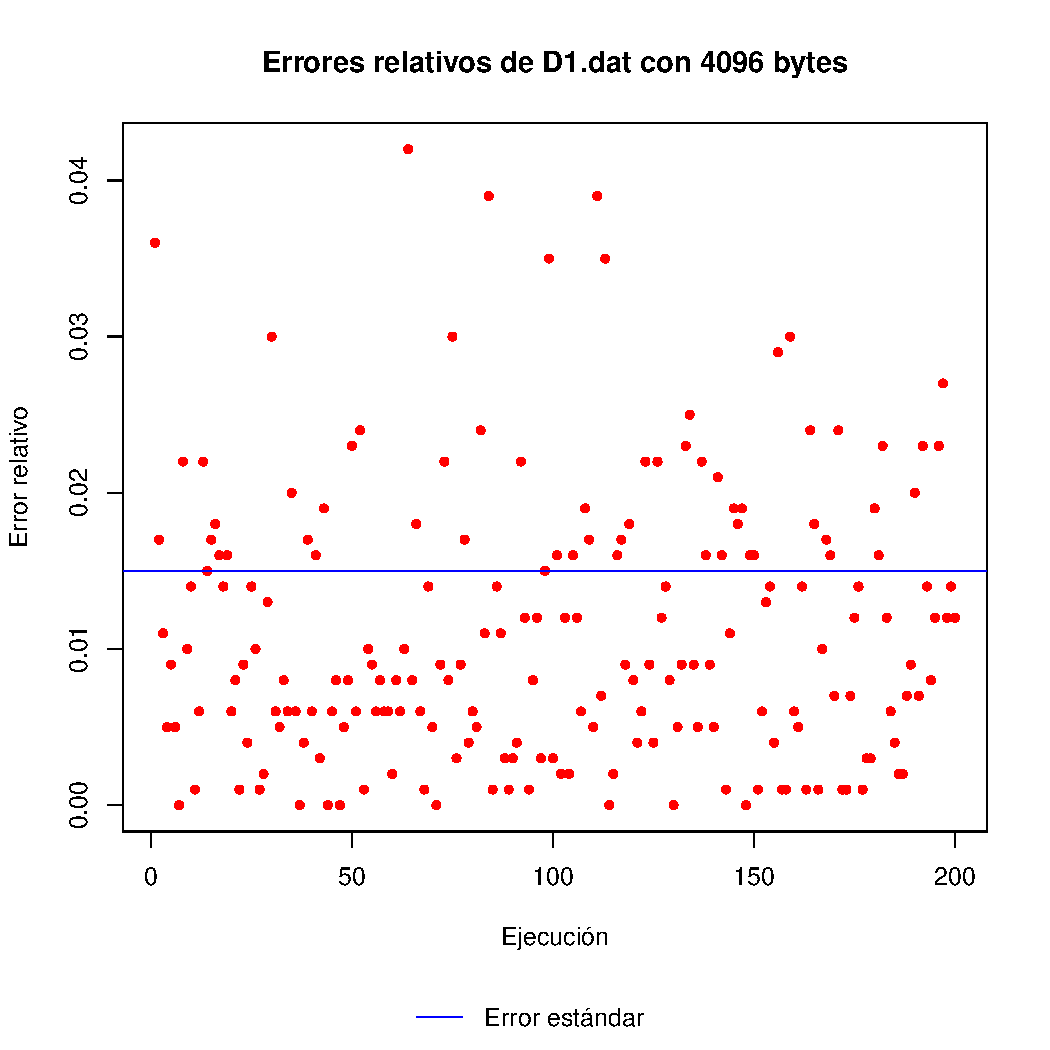
\includegraphics[width=0.64\textwidth]{../figs/D1/plot_errors_4096.pdf}
        \caption{Errores relativos en D1.dat con 4096 bytes}
    \label{figura:D1_errors_4096}
\end{figure}

\begin{figure}[h!]
    \centering
        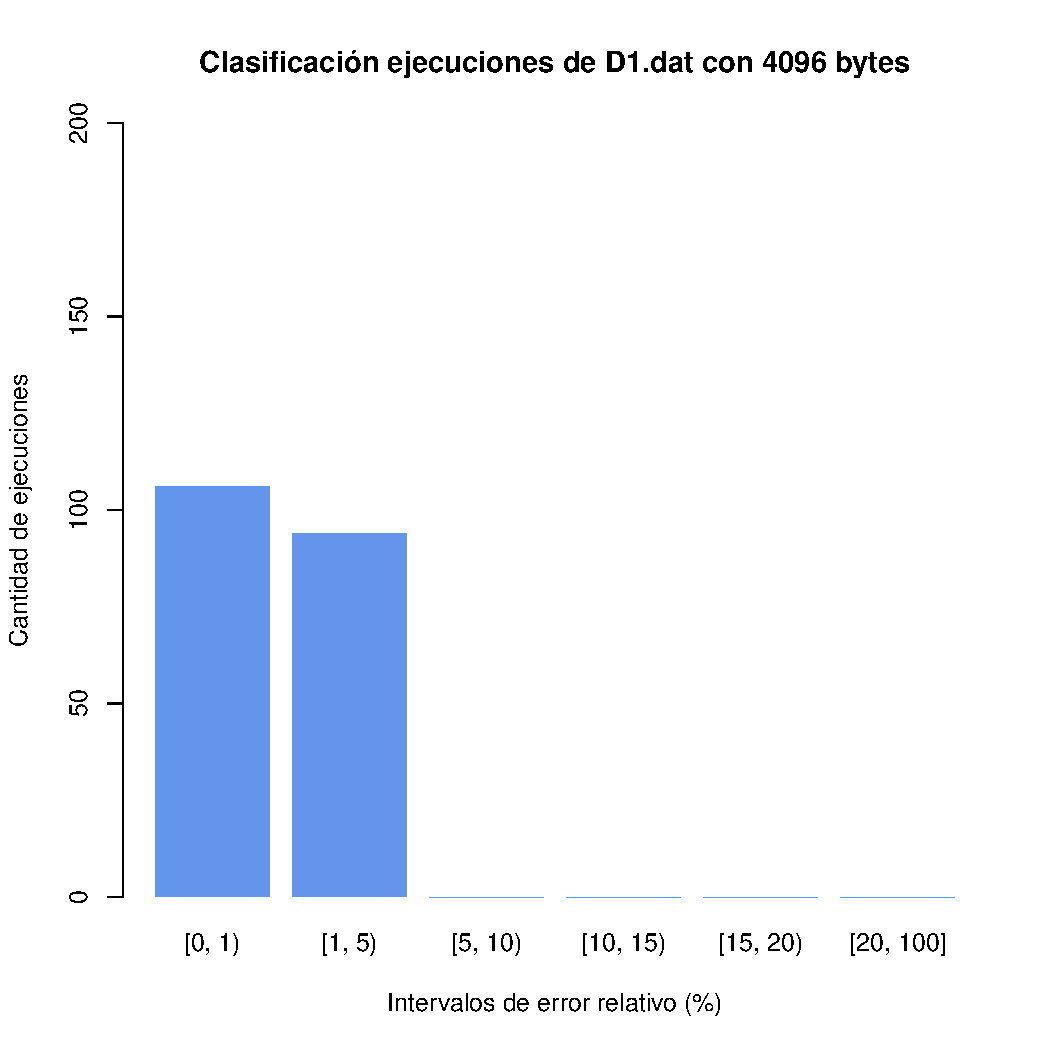
\includegraphics[width=0.64\textwidth]{../figs/D1/plot_count_4096.pdf}
        \caption{Clasificación de ejecuciones en D1.dat con 4096 bytes}
    \label{figura:D1_count_4096}
\end{figure}

\begin{figure}[h!]
    \centering
        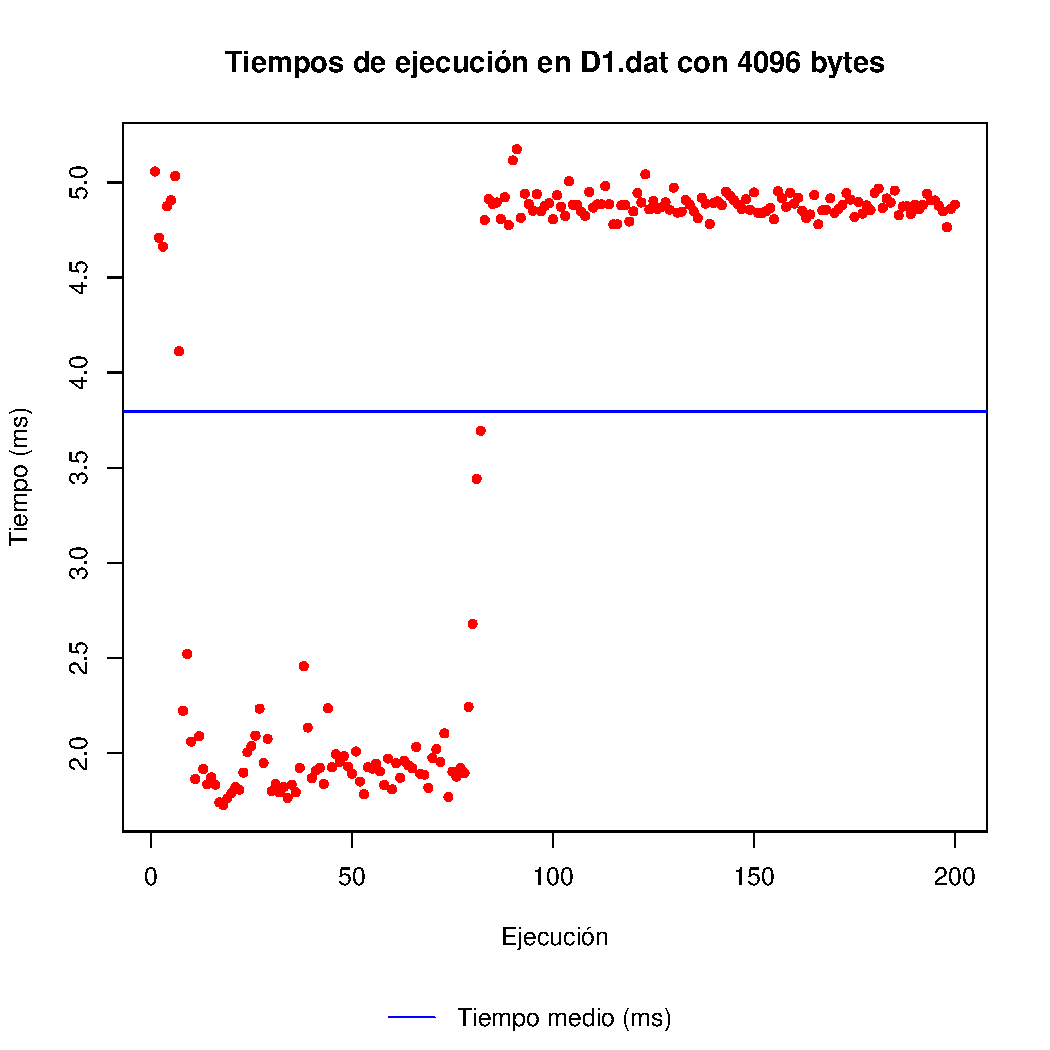
\includegraphics[width=0.64\textwidth]{../figs/D1/plot_time_4096.pdf}
        \caption{Tiempos de ejecución en D1.dat con 4096 bytes}
    \label{figura:D1_time_4096}
\end{figure}

\clearpage
\subsubsection{8192 bytes}
\begin{figure}[h!]
    \centering
        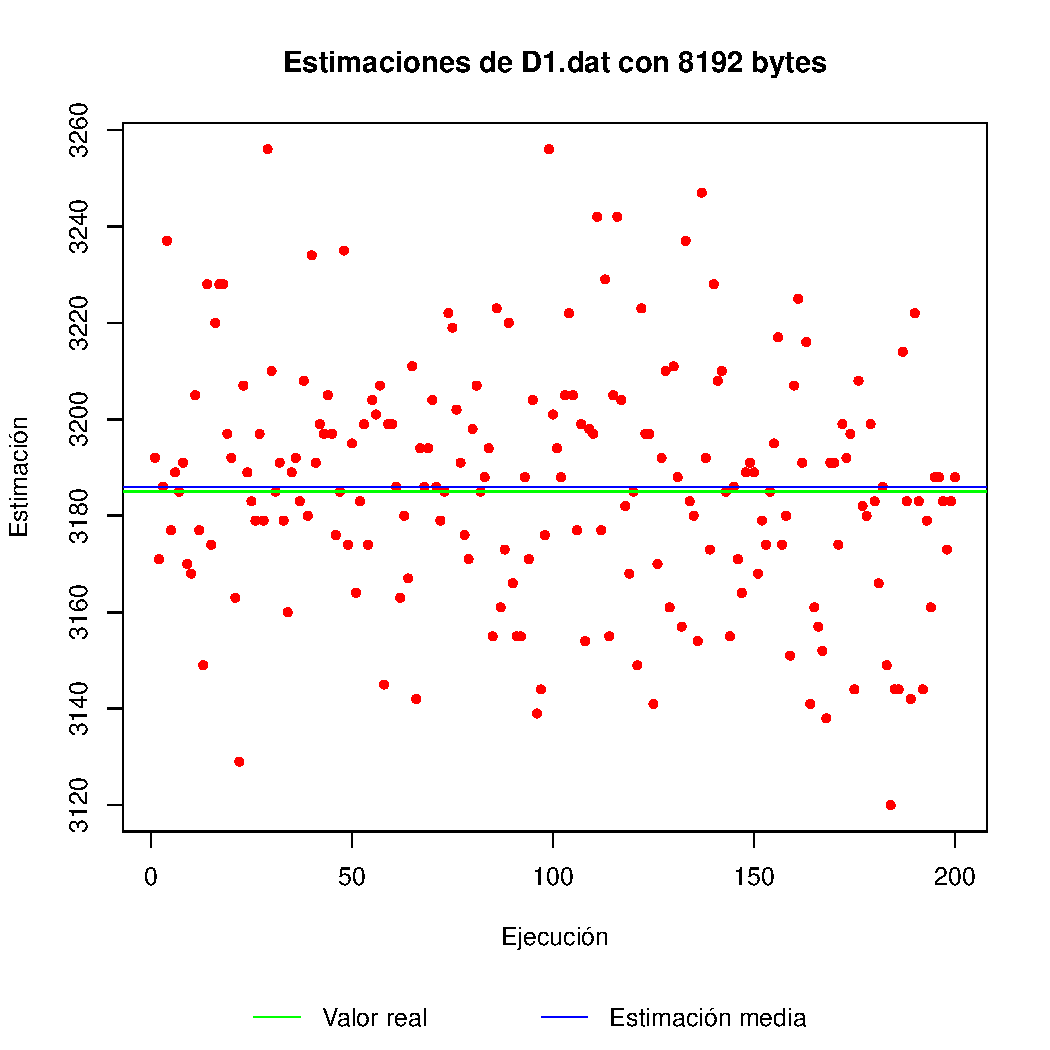
\includegraphics[width=0.64\textwidth]{../figs/D1/plot_estimation_8192.pdf}
        \caption{Estimaciones en D1.dat con 8192 bytes}
    \label{figura:D1_estimation_8192}
\end{figure}

\begin{figure}[h!]
    \centering
        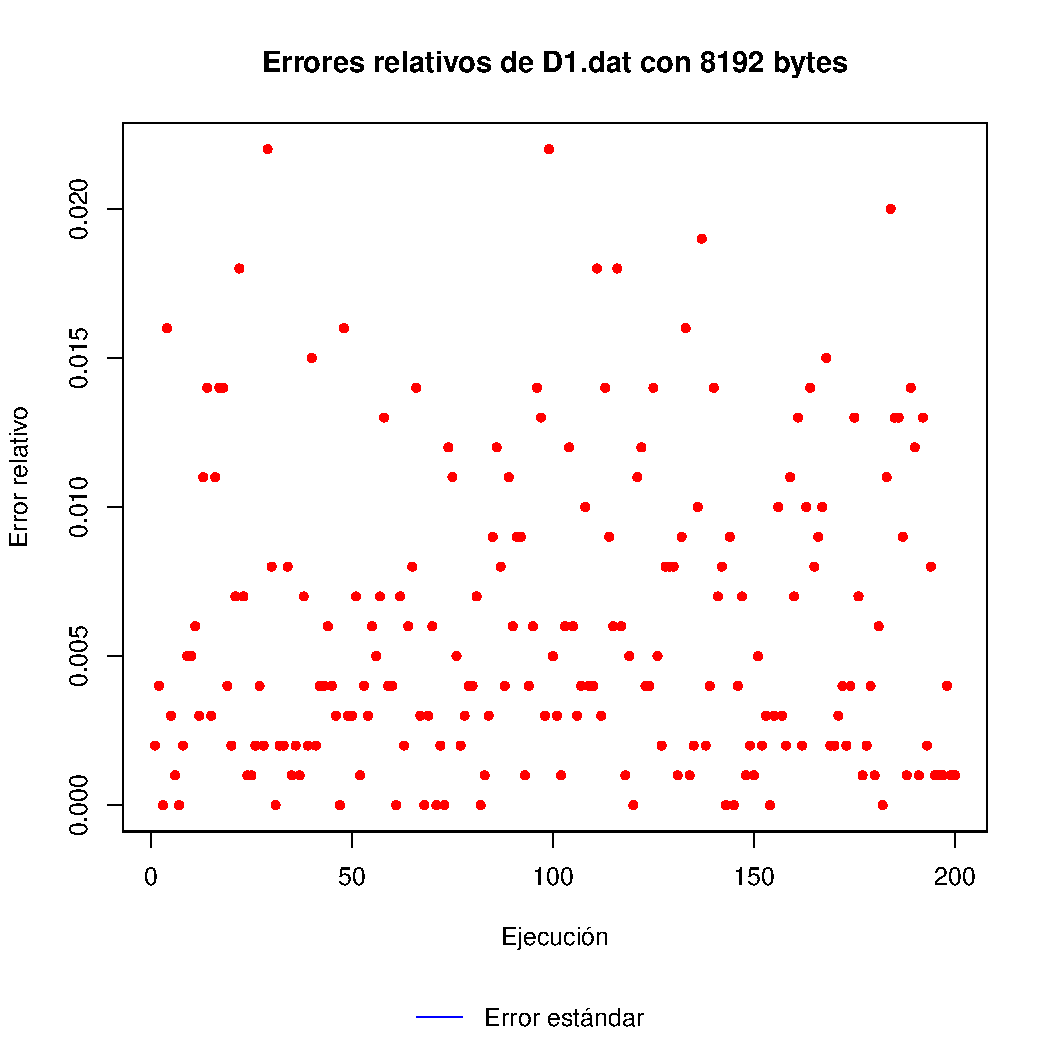
\includegraphics[width=0.64\textwidth]{../figs/D1/plot_errors_8192.pdf}
        \caption{Errores relativos en D1.dat con 8192 bytes}
    \label{figura:D1_errors_8192}
\end{figure}

\begin{figure}[h!]
    \centering
        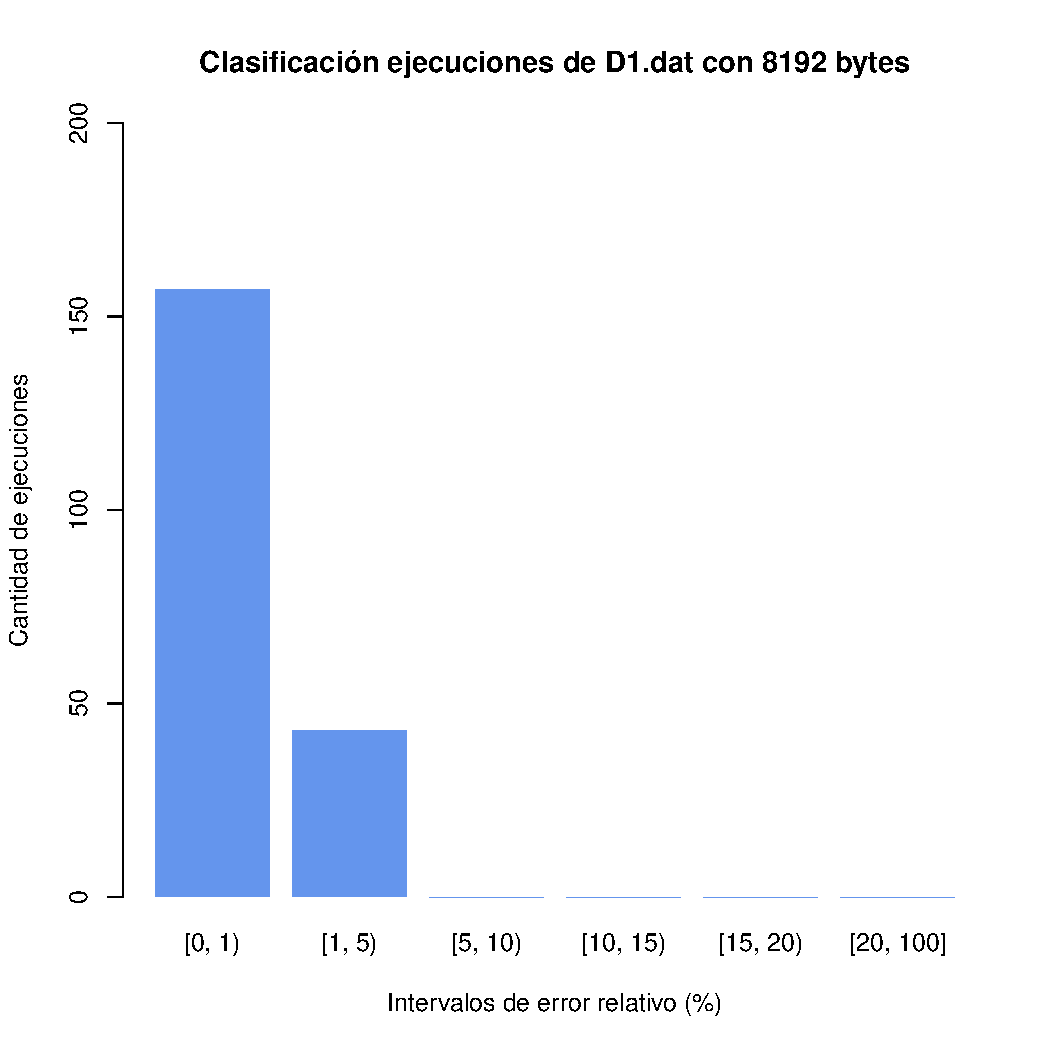
\includegraphics[width=0.64\textwidth]{../figs/D1/plot_count_8192.pdf}
        \caption{Clasificación de ejecuciones en D1.dat con 8192 bytes}
    \label{figura:D1_count_8192}
\end{figure}

\begin{figure}[h!]
    \centering
        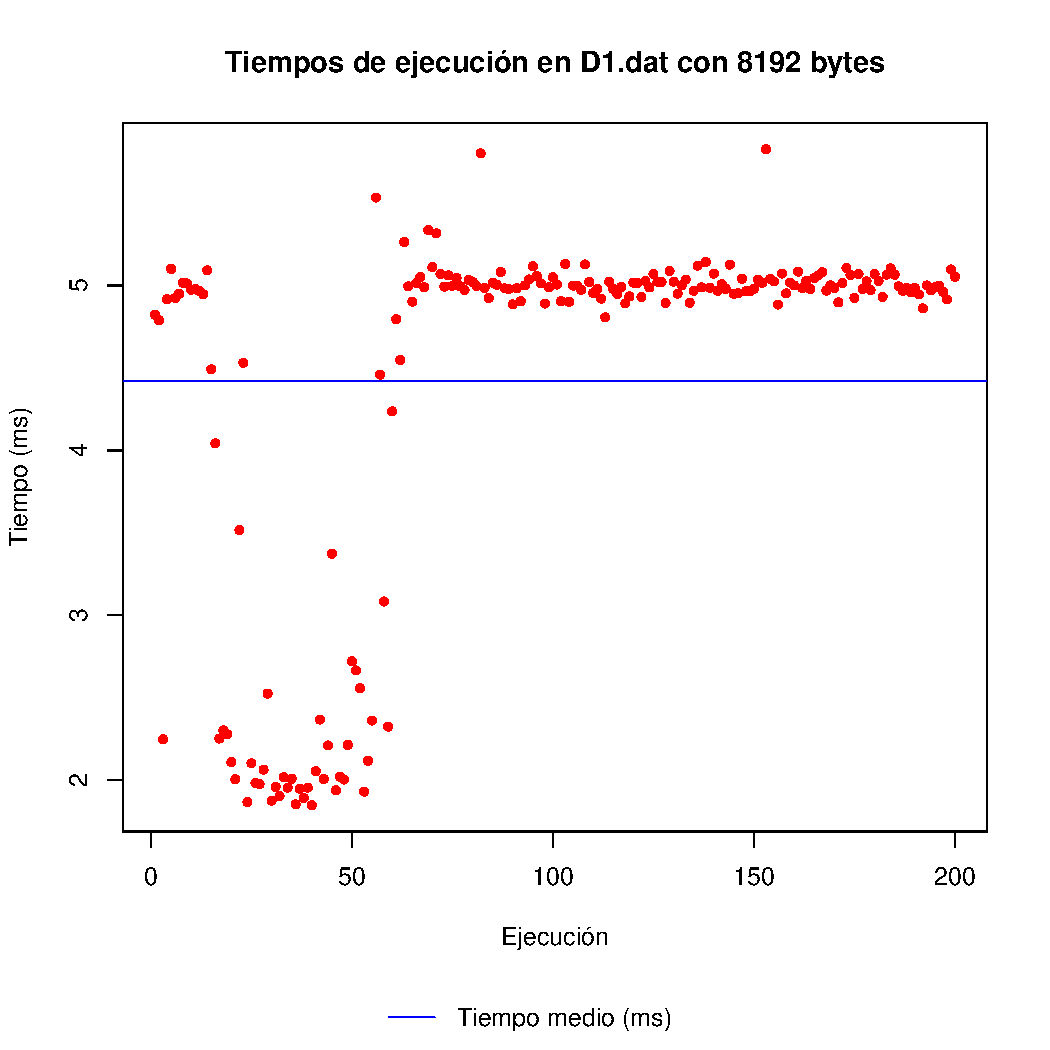
\includegraphics[width=0.64\textwidth]{../figs/D1/plot_time_8192.pdf}
        \caption{Tiempos de ejecución en D1.dat con 8192 bytes}
    \label{figura:D1_time_8192}
\end{figure}

\clearpage
\subsubsection{16384 bytes}
\begin{figure}[h!]
    \centering
        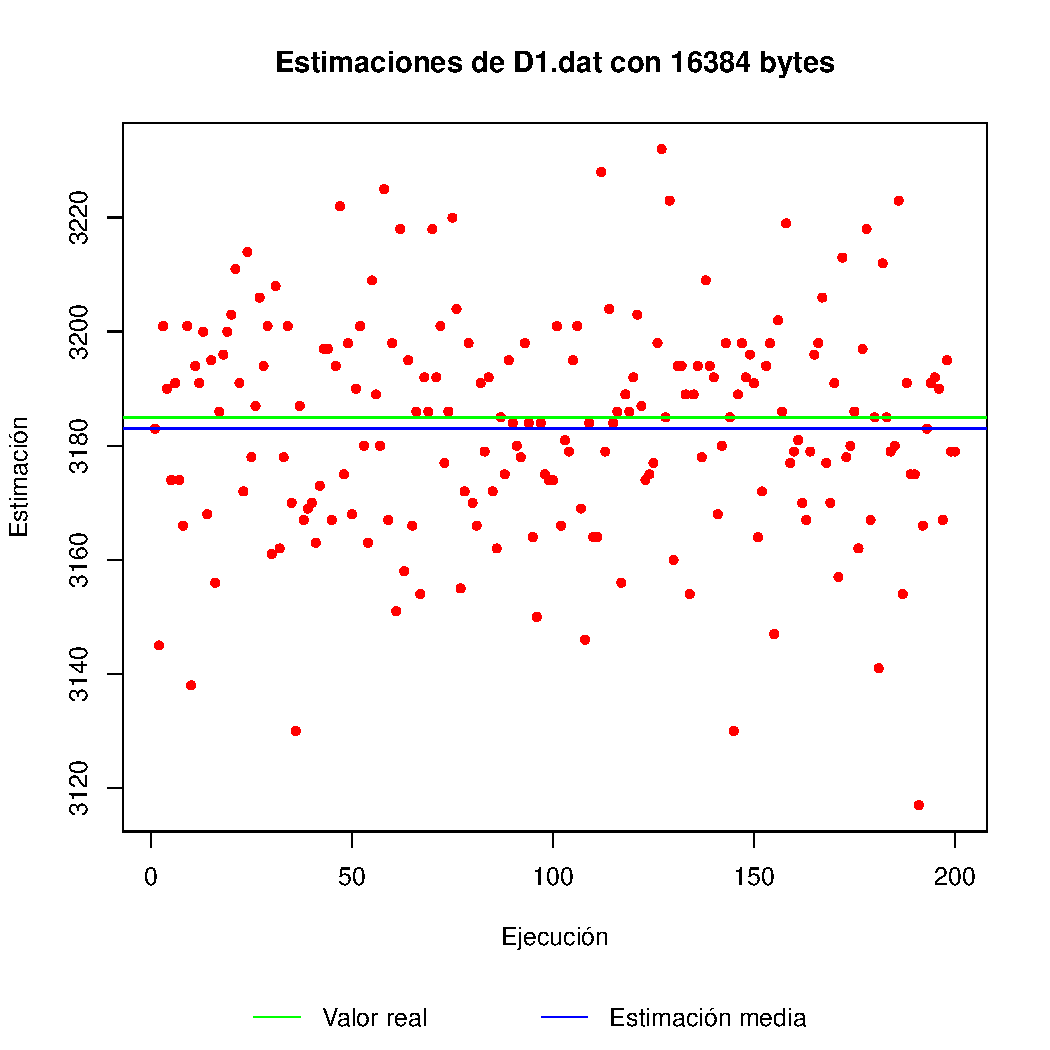
\includegraphics[width=0.64\textwidth]{../figs/D1/plot_estimation_16384.pdf}
        \caption{Estimaciones en D1.dat con 16384 bytes}
    \label{figura:D1_estimation_16384}
\end{figure}

\begin{figure}[h!]
    \centering
        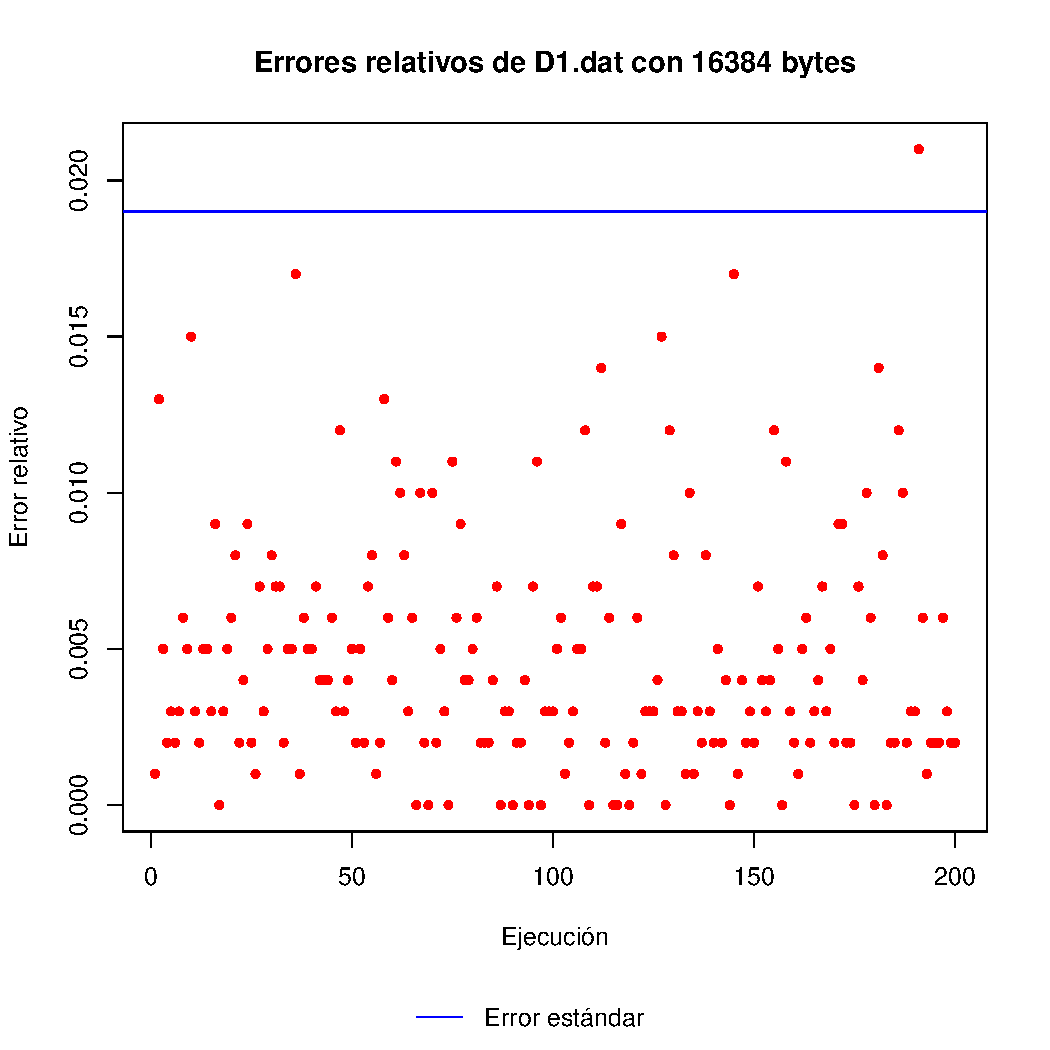
\includegraphics[width=0.64\textwidth]{../figs/D1/plot_errors_16384.pdf}
        \caption{Errores relativos en D1.dat con 16384 bytes}
    \label{figura:D1_errors_16384}
\end{figure}

\begin{figure}[h!]
    \centering
        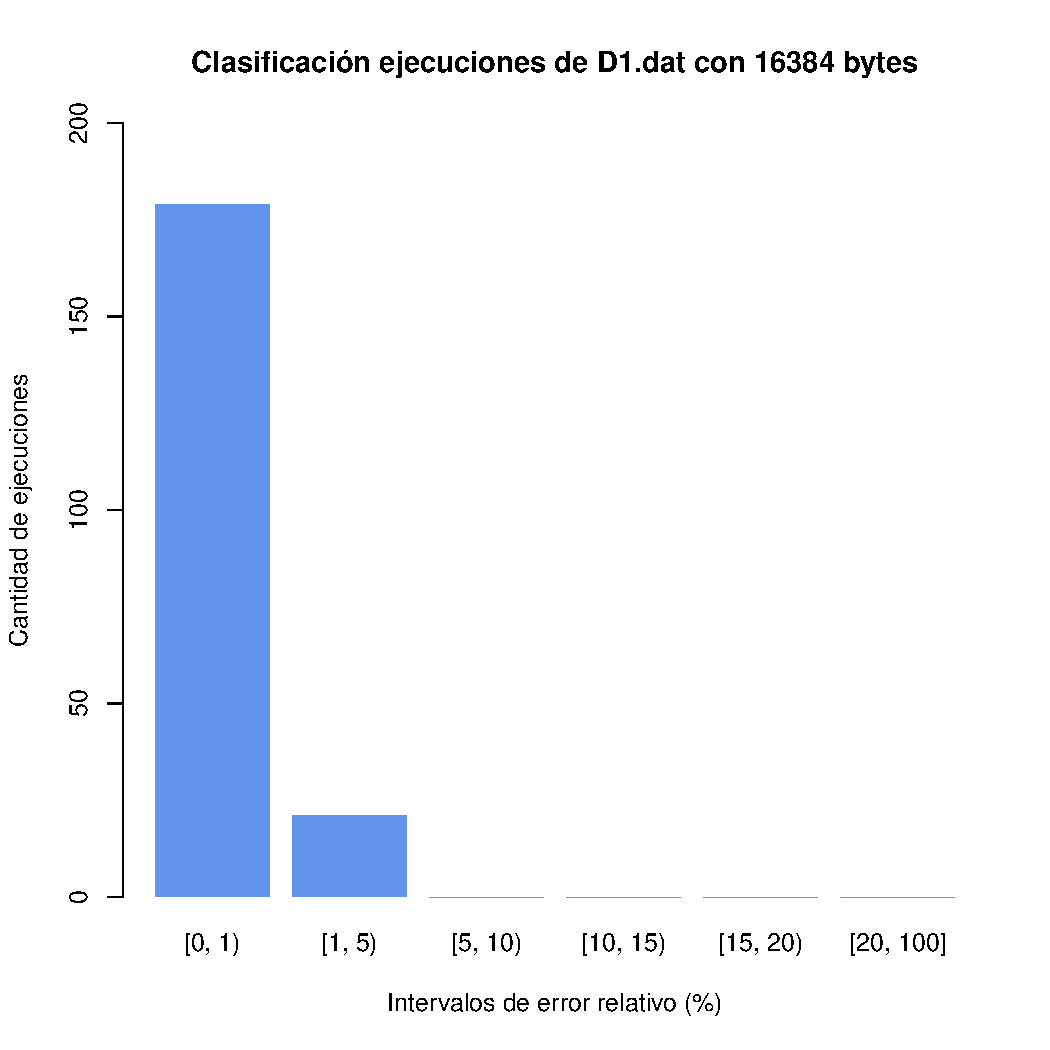
\includegraphics[width=0.64\textwidth]{../figs/D1/plot_count_16384.pdf}
        \caption{Clasificación de ejecuciones en D1.dat con 16384 bytes}
    \label{figura:D1_count_16384}
\end{figure}

\begin{figure}[h!]
    \centering
        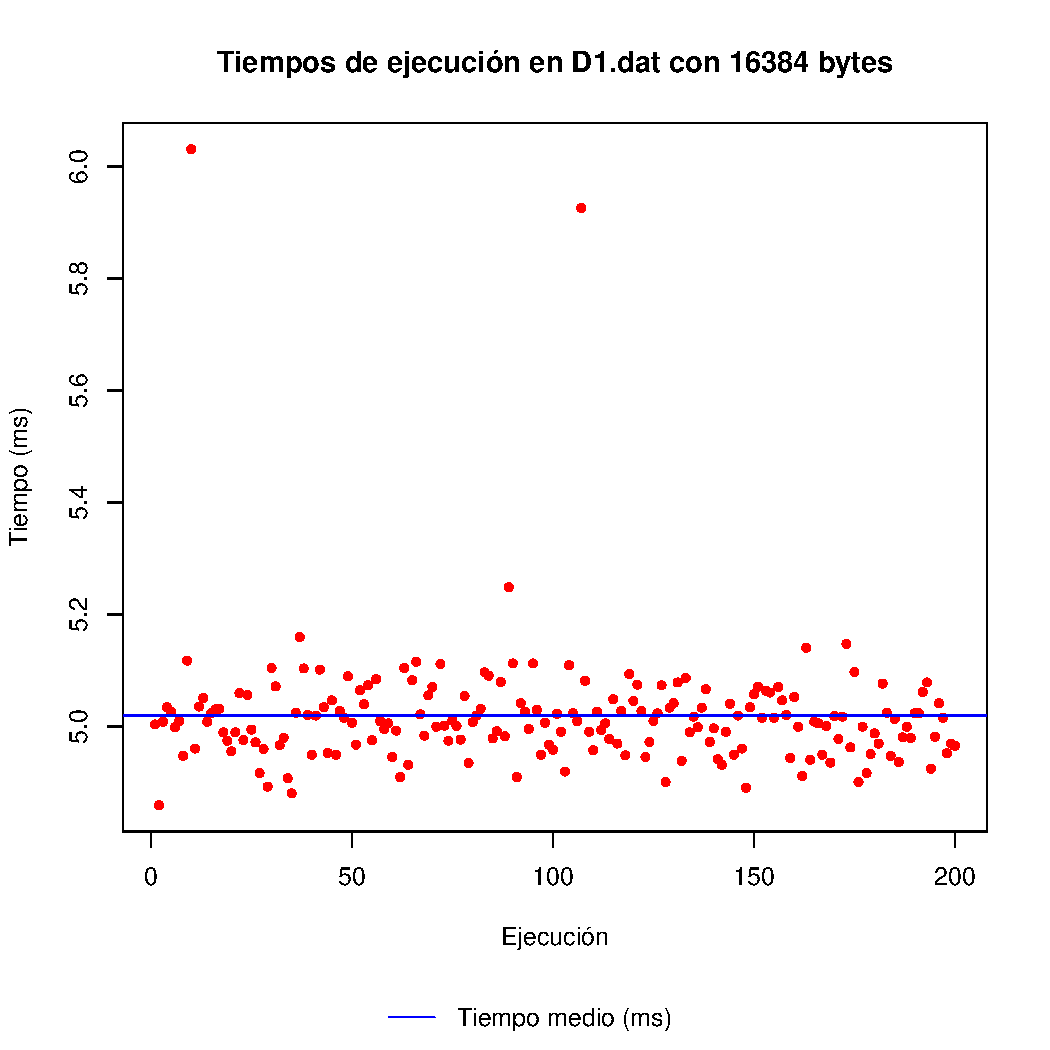
\includegraphics[width=0.64\textwidth]{../figs/D1/plot_time_16384.pdf}
        \caption{Tiempos de ejecución en D1.dat con 16384 bytes}
    \label{figura:D1_time_16384}
\end{figure}

\clearpage


\end{appendix}

\end{document}
